\documentclass[11pt]{article}
\usepackage[a4paper,margin=2.5cm]{geometry}
\usepackage[T1]{fontenc}
\usepackage{lmodern}
\usepackage[natbibapa]{apacite}
\renewcommand{\doiprefix}{https://doi.org/}
\usepackage{amsmath,amssymb,booktabs,graphicx,xcolor,algorithm,algpseudocode,longtable}
\usepackage[hidelinks]{hyperref}
\graphicspath{{figures/}}
\newcommand{\E}{\mathbb{E}}
\newcommand{\Prob}{\mathbb{P}}
\newcommand{\lord}{\ell_\lambda}
\renewcommand{\thesection}{S\arabic{section}}
\renewcommand{\thetable}{S\arabic{table}}
\renewcommand{\thefigure}{S\arabic{figure}}
\renewcommand{\thealgorithm}{S\arabic{algorithm}}
\title{Online Supplement to\\[3pt]
\textbf{Fair vehicle routing with random route durations: ex-post ordered
fairness, rank prices and risk-consistent tours}}
\author{Quang-Vinh Dang, Hoang-Viet Vu, Phuc-Son Nguyen}
\date{}
\begin{document}
\maketitle
\noindent This supplement contains the detailed pseudocode and parameters of
the algorithm (Section~\ref{sec:salg}), the complete computational study with
all seventeen experiments E1--E17 and their tables and figures
(Section~\ref{sec:sexp}), and per-instance results
(Section~\ref{app:tables}). Numbers of sections, propositions, theorems,
tables and figures without the prefix S refer to the main paper.

\section{Algorithm details}\label{sec:salg}
Algorithm~\ref{alg:improve} details the improvement step of the main loop
(Algorithm~1 of the main paper), and Table~\ref{tab:params} lists all
parameters; they are identical for all methods and instances.

\begin{algorithm}[t]
\caption{\textsc{ImproveStep}$(P,\varpi,\psi)$: screen, evaluate, confirm}\label{alg:improve}
\begin{algorithmic}[1]
\For{every relocate $(i:a\to b)$ and swap $(i\in a,\,j\in b)$}
  \State compute insertion and removal deltas $\Delta L_a,\Delta L_b,\Delta W_a,\Delta W_b$
  \If{capacity holds and $\sum_kL_k+\Delta L_a+\Delta L_b\le(1+\epsilon_B)\,B\,C^\ast$}
    \State $\hat\Delta\gets\varpi_a\Delta L_a+\varpi_b\Delta L_b+\psi_a\Delta\sigma_a+\psi_b\Delta\sigma_b$ \Comment{eq.~the prediction formula of Section~5.3}
  \EndIf
\EndFor
\State $\mathcal K\gets$ the $K$ moves with the smallest $\hat\Delta$
\For{each move in $\mathcal K$} \State re-solve routes $a,b$ with \emph{screening} tours; evaluate $F$ by PBOI \EndFor
\For{each improving candidate, best first}
  \State re-solve routes $a,b$ with the \emph{exact} lower level; re-evaluate $F$
  \If{$F$ still improves and $\sum_kL_k\le B\,C^\ast$} \Return the confirmed plan \EndIf
\EndFor
\State \Return \textsc{none}
\end{algorithmic}
\end{algorithm}

\begin{table}[t]\centering\small
\caption{Parameters of SORTIE (identical for all methods and instances).}\label{tab:params}
\begin{tabular}{llr}
\toprule
Component & Parameter & Value\\
\midrule
Lower level & exact Held--Karp up to & 15 customers\\
 & local-search starts beyond that & 8\\
 & screening tours & 1 descent, $\le$24 tours if $\kappa>0$\\
Evaluator & Gauss--Legendre points per panel / quantile levels & 6 / 13\\
 & dispersion-price step & $0.05\,\sigma_k$\\
Screen & candidates evaluated per step $K$ & 8\\
 & budget slack in the screen $\epsilon_B$ & 2\%\\
Ruin & removed customers $q$ & $2$ to $\max(3,\min(12,\lceil n/4\rceil))$\\
 & price-weighted pool / related removal & probability $1/2$ each\\
Recreate & cost tie-breaker in $s_b(i)$ & $10^{-3}$\\
Repair & maximum cost-descent steps & 200\\
Annealing & initial temperature / final ratio & $0.02\,|F(P_0)|$ / $10^{-3}$\\
\bottomrule
\end{tabular}
\end{table}


\section{Extended computational study}\label{sec:sexp}

\subsection{Set-up}
\paragraph{Instances.} We follow the slicing rule of the deterministic fair
routing literature \citep{ljubic2026fair}. Block $b$ of size $n$ consists of the
depot and the $n$ consecutive customers $bn+1,\dots,(b+1)n$ of CVRPLIB
X-n641-k35 \citep{uchoa2017new}, with ceiled Euclidean distances, $m=5$
vehicles and capacity $Q=\lfloor\sum_i q_i/4\rfloor$, so one vehicle's worth
of slack is available. The main grid uses $n\in\{15,20,25,30,35\}$ and blocks
$b=0,\dots,4$ (25 instances); the scale test uses $n\in\{50,75,100\}$ and
blocks $0$--$5$; the exactness test uses ten instances with $n=10$, $m=3$ and
$Q=\lfloor\sum_i q_i/2.4\rfloor$.

\paragraph{Uncertainty.} Unless stated otherwise $v=0.3$ (gamma arc noise) and
$s_Y=0.15$. In the congestion experiment (E8) the arc coefficient of variation
is $vH_{ij}$, where $H_{ij}\in[1/3,2]$ is largest for arcs near a randomly
drawn congestion centre, so noise is no longer proportional to length.

\paragraph{Budget.} $C^\ast$ is the cost of the best of three restarts of
the cost-minimising search; the total length of every fair plan must satisfy
$\sum_k L_k\le B\,C^\ast$ with $B\in\{1.05,1.10\}$.

\paragraph{Methods.} All methods share the search of Algorithm~1,
the start plan, the time limit (15\,s for $n\le25$, 25\,s for $n\ge30$, 120\,s
for $n\ge50$) and the random seed. They differ only in the objective and in the
lower level.
\emph{Det} minimises the deterministic ordered measure $\lord(L)$ of the tour
lengths, i.e.\ the model of \citet{ljubic2026fair} solved heuristically.
\emph{SAA} minimises the sample average of $\lord(X)$ over 200 fixed arc
scenarios. \emph{SORTIE-0} minimises the exact ex-post value by PBOI with
TSP-optimal tours ($\kappa=0$); \emph{SORTIE-1} uses the risk-consistent lower
level with $\kappa=1$. In Det and SAA the moves are screened by the
deterministic and the sample objective respectively.

\paragraph{Evaluation.} Every plan is evaluated out of sample by arc-level
Monte Carlo with $20\,000$ scenarios ($10\,000$ for $n\ge 50$), including the
day factor, with common random numbers across methods. The reported
\emph{ex-post value} is the Monte Carlo estimate of $\E\lord(\Phi)$. Paired
comparisons use the Wilcoxon signed-rank test. All tables are generated from
the raw results by the released scripts.

\subsection{Accuracy and cost of the evaluator (E1, E2)}
Table~\ref{tab:e1} compares PBOI with $50\,000$-sample arc-level Monte Carlo
on 168 plans: the cost-efficient plans and random feasible plans whose
routes are sequenced by the lower level, for $n\in\{15,25,35,50\}$. The mean absolute
relative error is below $0.11\%$ for all five measures and at most $0.44\%$ in
the worst case, and 99--100\% of the differences lie within three Monte Carlo
standard errors. The mean $z$-scores are not exactly zero (up to $0.34$ for the
MAD): PBOI carries a systematic bias of a few hundredths of a percent, which
we attribute to the moment-matched gamma marginal of each route (a sum of arc
gammas with different scales is not exactly gamma). PBOI takes $0.44$\,ms per plan for $m=5$, against
$0.28$\,s for $20\,000$-scenario Monte Carlo. A 200-scenario SAA is about
seven times faster than PBOI but is a noisy estimate. The advantage of PBOI is
therefore that it is exact and noise-free at a cost compatible with thousands
of evaluations per second, not raw speed.

\begin{table}[t]\centering\small
\caption{E1: PBOI against arc-level Monte Carlo ($50\,000$ samples) on 168 plans; $z$: difference over its Monte Carlo standard error.}\label{tab:e1}
\begin{tabular}{lrrrr}\toprule
Measure & Plans & Mean $|$err$|$ (\%) & Max $|$err$|$ (\%) & Share $|z|<3$ \\
\midrule
Max & 168 & 0.041 & 0.137 & 0.994 \\
Range & 168 & 0.062 & 0.249 & 1.000 \\
GMD & 168 & 0.057 & 0.241 & 1.000 \\
MAD & 168 & 0.064 & 0.272 & 0.988 \\
Var & 168 & 0.108 & 0.440 & 0.994 \\
\bottomrule
\end{tabular}

\end{table}

On the ten $n=10$ instances we enumerated all capacity- and budget-feasible
partitions (4 to 145 per instance) with exact Held--Karp tours. The cost
search found the optimal $C^\ast$ on all ten. For both range and GMD, SORTIE-0
found the plan with the smallest exact ex-post value on nine of ten
instances (mean gap $0.39\%$, maximum $3.9\%$). Det found the deterministic
optimum on nine of ten; on the tenth instance, which has only 20
budget-feasible partitions, it stopped at a plan with twice the optimal
deterministic range.

\subsection{The fairness illusion and the value of ex-post optimisation (E3)}
Table~\ref{tab:illusion} quantifies Proposition~9. A
deterministic fair plan believes its unfairness is the ex-ante value, which
understates the true ex-post value by $8\%$ for the maximum, $15$--$18\%$ for
the range, GMD and MAD, and $27\%$ for the variance. The in-sample SAA value is optimistic by
about $1\%$, which is the optimiser's curse on 200 scenarios. The PBOI value
believed by SORTIE has a mean signed error below $0.1\%$, a mean absolute
error of $0.07$--$0.23\%$ and a worst case of $1\%$.

\begin{table}[t]\centering\small
\caption{E3: what each method believes its unfairness is, relative to the
true ex-post value (Monte Carlo without the day factor, which is what each
model represents), mean signed error over 50 runs per cell. Last column:
largest absolute error of the PBOI prediction for any method's plan.}\label{tab:illusion}
\begin{tabular}{lrrrrr}\toprule
 & \multicolumn{4}{c}{Believed vs true (mean signed \%)} & PBOI \\
Measure & Det & SAA & SORTIE-0 & SORTIE-1 & max $|$err$|$ \% \\
\midrule
Max & -7.97 & -0.71 & -0.01 & -0.01 & 0.20 \\
Range & -17.56 & -0.99 & +0.03 & +0.02 & 0.70 \\
GMD & -14.68 & -0.91 & +0.04 & +0.05 & 0.61 \\
MAD & -16.17 & -0.88 & +0.05 & +0.07 & 0.68 \\
Var & -27.23 & -1.33 & +0.00 & +0.02 & 0.98 \\
\bottomrule
\end{tabular}

\end{table}

Table~\ref{tab:e3} reports the out-of-sample ex-post value relative to Det.
The signed-rank test favours SORTIE-0 and SORTIE-1 over Det in 9 of the 10
cells each. Pooled over all 250 runs, SORTIE-0 improves on Det by $0.89\%$ on
average (median $0.23\%$; better in 141 runs, tied in 96, worse in 13;
$p<10^{-18}$) and SORTIE-1 by $0.77\%$ (better in 154, worse in 31). SAA
improves by only $0.14\%$ (median zero; better in 115, worse in 74) and is
favoured significantly in 3 cells. Head to head, SORTIE-0 beats SAA in 145
runs and loses in 15, and SORTIE-1 beats it in 147 and loses in 27
($p<10^{-17}$). The largest gains are for the maximum at
$B=1.10$ ($2.1\%$, 24 of 25 instances), where the extra budget lets the
planner trade a slightly longer but less variable longest route.

The improvements are small, about one percent on average, and this is itself
a finding. With homogeneous
noise ($\sigma_k^2=v^2W_k$) the standard deviation of a route grows with its
length, so the plans that balance lengths also nearly balance risks, and a
deterministic fair plan is close to ex-post optimal even though its
\emph{assessment} of its own fairness is badly wrong. For context, the
cost-optimal plan has an ex-post range of 2087 against about 1340 for the fair
plans, at a cost $6.5\%$ higher: fairness itself is worth optimising; the
stochastic refinement adds about one percent on top. For range-optimised plans
the CVaR$_{0.9}$ of the realised range, which none of the methods optimises, is
2054 for Det, 2059 for SAA, 2037 for SORTIE-0 and 2032 for SORTIE-1; both
SORTIE variants improve it at both budgets, SAA at neither.

\begin{table}[t]\centering\small
\caption{E3: improvement of the out-of-sample ex-post value over Det (mean
\%, positive is better; in brackets the number of instances on which the
method is strictly better). $^\ast$: Wilcoxon signed-rank $p<0.05$ in favour
of the method; the test is on ranks and can disagree in sign with the mean
when one instance dominates (Var, $B=1.10$, SORTIE-1).}\label{tab:e3}
\begin{tabular}{llrrr}\toprule
Measure & $B$ & SAA & SORTIE-0 & SORTIE-1 \\
\midrule
GMD & 1.05 & -0.40 (6/25) & -0.09 (8/25) & -0.03 (9/25) \\
GMD & 1.10 & -0.32 (9/25) & +0.94$^\ast$ (14/25) & +0.34$^\ast$ (17/25) \\
MAD & 1.05 & +0.86$^\ast$ (11/25) & +1.10$^\ast$ (13/25) & +1.24$^\ast$ (12/25) \\
MAD & 1.10 & +0.70 (13/25) & +0.96$^\ast$ (14/25) & +1.53$^\ast$ (18/25) \\
Max & 1.05 & +0.71$^\ast$ (14/25) & +0.61$^\ast$ (15/25) & +0.77$^\ast$ (15/25) \\
Max & 1.10 & +1.70$^\ast$ (23/25) & +2.08$^\ast$ (24/25) & +1.93$^\ast$ (24/25) \\
Range & 1.05 & +0.12 (13/25) & +0.64$^\ast$ (15/25) & +1.56$^\ast$ (15/25) \\
Range & 1.10 & -0.21 (13/25) & +1.07$^\ast$ (17/25) & +0.39$^\ast$ (15/25) \\
Var & 1.05 & +0.48 (7/25) & +0.50$^\ast$ (9/25) & +0.48$^\ast$ (13/25) \\
Var & 1.10 & -2.25 (6/25) & +1.09$^\ast$ (12/25) & -0.49$^\ast$ (16/25) \\
\bottomrule
\end{tabular}

\end{table}

\begin{figure}[t]\centering
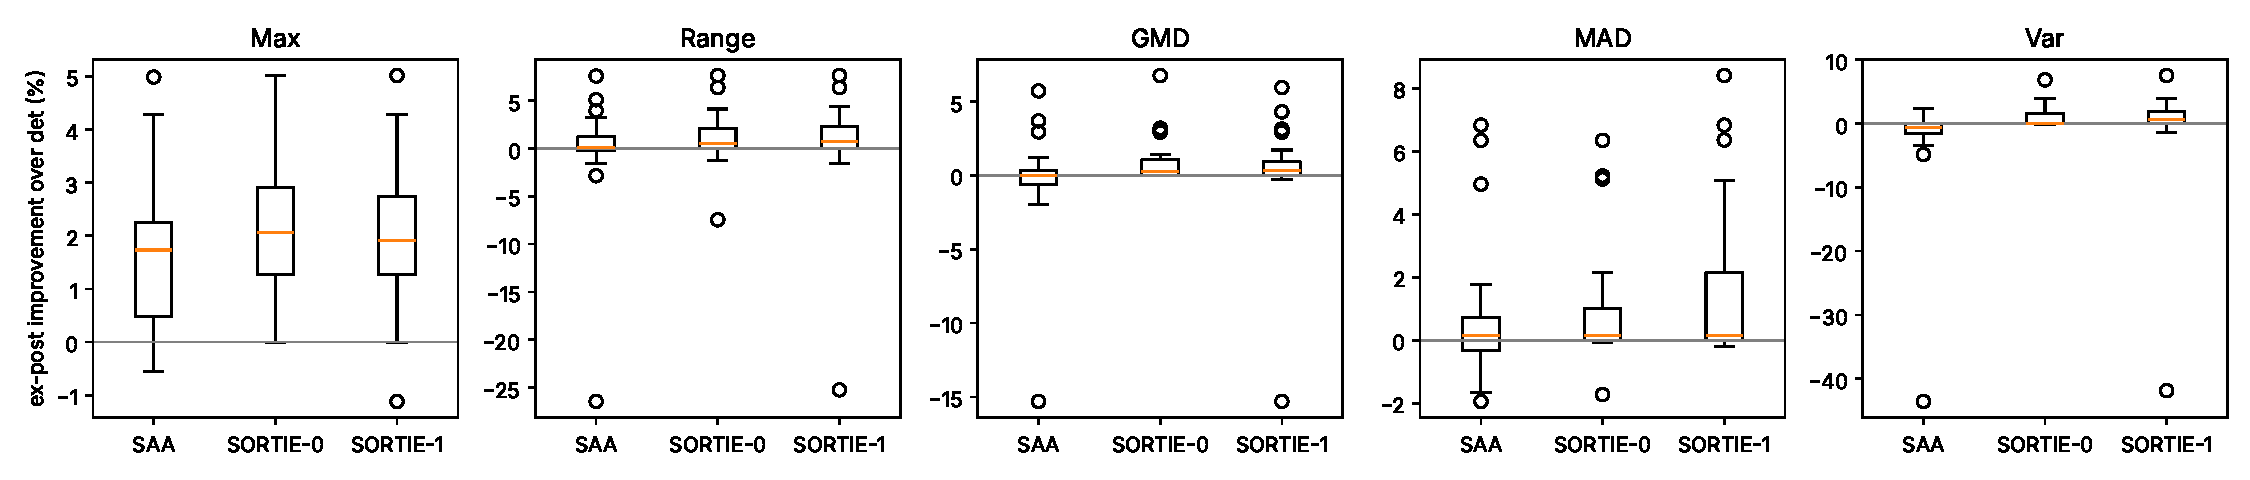
\includegraphics[width=\textwidth]{e3_improvement.pdf}
\caption{E3, $B=1.10$: per-instance improvement of the ex-post value over Det.}\label{fig:e3}
\end{figure}

\paragraph{An illustrative instance.} Figure~\ref{fig:routes} shows the
cost-optimal plan and the range-optimised Det and SORTIE-0 plans of
X641-n30-b0 at $B=1.10$, an instance whose SORTIE-0 gain ($+0.47\%$) is
close to the median of the 25 instances ($+0.54\%$). The cost plan leaves one driver with a
route of length 148 and another with 2610. Both fair plans balance the
lengths to a deterministic range of about 940, and they differ only in how
two route pairs are split. Figure~\ref{fig:workloads} shows what the drivers
experience. The realised workloads are wide and right-skewed, and the
expected realised range is about 1225 for both fair plans: 30\% above the
deterministic range the Det planner reports. Figure~\ref{fig:rangedist} gives
the distribution of the realised range of the two plans; in one day out of
ten it exceeds 1750. The worst instance for SORTIE-0 in this cell is
X641-n35-b0, where Det is $7.5\%$ better (Figure~\ref{fig:heatmap} in
Appendix~\ref{app:tables}); this is consistent with the search noise
documented in E7b rather than a systematic effect, since on the same instance
SORTIE-0 is better or tied in eight of the other nine cells.

\begin{figure}[t]\centering
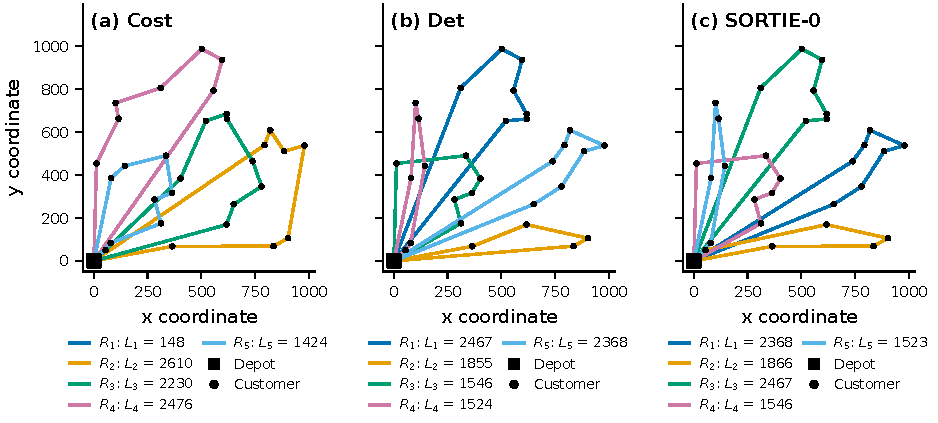
\includegraphics[width=\textwidth]{fig_routes.pdf}
\caption{X641-n30-b0, $B=1.10$: cost-optimal plan and the range-optimised Det
and SORTIE-0 plans. $L_k$: tour lengths.}\label{fig:routes}
\end{figure}

\begin{figure}[t]\centering
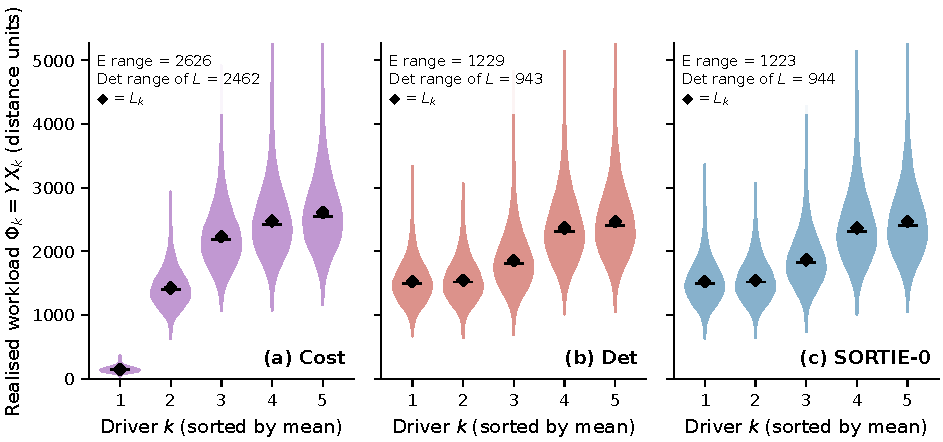
\includegraphics[width=\textwidth]{fig_workloads.pdf}
\caption{Simulated realised workloads $\Phi_k=YX_k$ of the three plans of
Figure~\ref{fig:routes} ($20\,000$ days); diamonds mark the tour lengths
$L_k$ that a deterministic model sees.}\label{fig:workloads}
\end{figure}

\begin{figure}[t]\centering
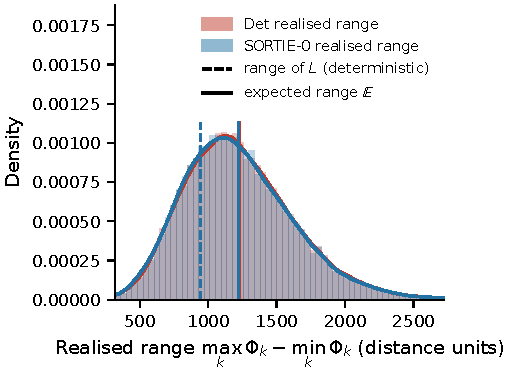
\includegraphics[width=0.6\textwidth]{fig_rangedist.pdf}
\caption{Distribution of the realised range of the Det and SORTIE-0 plans of
Figure~\ref{fig:routes}; dashed: deterministic range of the tour lengths,
solid: expected realised range.}\label{fig:rangedist}
\end{figure}

\paragraph{How tight is the illusion bound?} Figure~\ref{fig:bound} plots the
gap between the true ex-post value and the ex-ante value of every Det plan
against the bound of Proposition~9. No plan violates the bound.
The bound is conservative: the realised gap is on average $33\%$ of the
bound for the maximum, $18\%$ for the range and $11$--$12\%$ for the GMD and
MAD, because it charges every route its full standard deviation while only
the routes near the extreme ranks matter. Its value is that it is computable
from the quadratic lengths alone and grows like $v\sqrt{\sum_kW_k}$, which is
the scaling observed in E6.

\begin{figure}[t]\centering
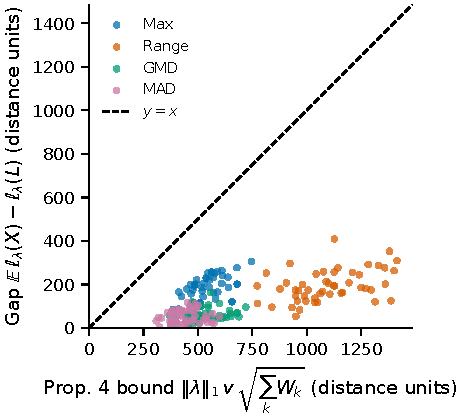
\includegraphics[width=0.6\textwidth]{fig_illusion_bound.pdf}
\caption{Fairness illusion of the Det plans of E3 (true ex-post minus
ex-ante value) against the bound $\|\lambda\|_1v(\sum_kW_k)^{1/2}$ of
Proposition~9.}\label{fig:bound}
\end{figure}

\begin{figure}[t]\centering
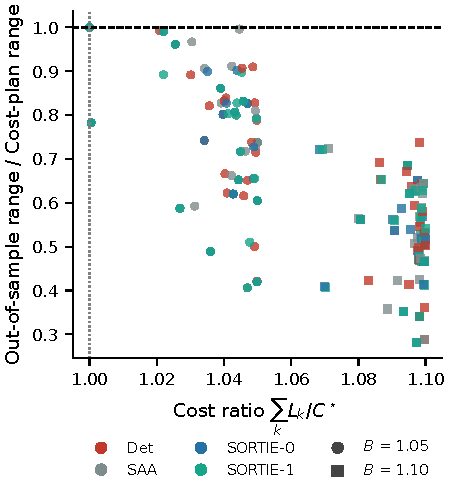
\includegraphics[width=0.6\textwidth]{fig_cost_fairness.pdf}
\caption{E3, range-optimised plans: total length relative to $C^\ast$ against
the expected realised range relative to that of the cost-optimal plan.}\label{fig:costfair}
\end{figure}

\subsection{Route consistency (E4)}
E4 removes the lower level: the planner may sequence each route freely
(\emph{free}) instead of using the TSP-optimal tour (\emph{lower}). For the
maximum, free sequencing changes almost nothing, as monotonicity predicts in
the deterministic case. For the range and the GMD the free planner lengthens
the short routes: 23 of 25 Det plans and 24 of 25 SORTIE plans for the range
contain a route that is not a shortest tour of its customers; the excess
length is 95 (Det) and 113 (SORTIE) distance units on average over the runs
that have one. This lowers the ex-post value by $1$--$3\%$ for Det
on both measures and for SORTIE on the range (Table~\ref{tab:e4}); for SORTIE
on the GMD it is $0.9\%$ worse, because the larger space slows the search. Wherever it helps, the reduction
comes from making some drivers drive detours. This is exactly the behaviour signalled by negative rank prices
and excluded by the bilevel constraint. The deterministic belief error persists
with free tours ($-24\%$ for the range); the PBOI belief remains exact.

\begin{table}[t]\centering\small
\caption{E4: free tours against lower-level tours, $B=1.10$, 25 instances per
row. $^a$Runs with at least one route that is not a shortest tour of its
customers. $^b$Mean number of such routes. Excess: total length above the
shortest tours of the same customer sets. Belief err: believed minus true
ex-post value. Ex-post: out-of-sample ex-post value.}\label{tab:e4}
\begin{tabular}{llrrrrr}\toprule
Measure & Method & Runs$^a$ & Routes$^b$ & Excess & Belief err (\%) & Ex-post \\
\midrule
Max & Det-lower & 0/25 & 0.00 & 0.0 & -8.94 & 2221.0 \\
Max & Det-free & 0/25 & 0.00 & 0.0 & -9.01 & 2232.4 \\
Max & SORTIE-lower & 0/25 & 0.00 & 0.0 & -0.00 & 2174.8 \\
Max & SORTIE-free & 7/25 & 0.36 & 2.7 & +0.00 & 2177.1 \\
Range & Det-lower & 0/25 & 0.00 & 0.0 & -23.11 & 1099.7 \\
Range & Det-free & 23/25 & 1.00 & 87.8 & -24.19 & 1088.5 \\
Range & SORTIE-lower & 0/25 & 0.00 & 0.0 & +0.04 & 1098.4 \\
Range & SORTIE-free & 24/25 & 1.64 & 108.4 & +0.06 & 1072.6 \\
GMD & Det-lower & 0/25 & 0.00 & 0.0 & -19.46 & 437.7 \\
GMD & Det-free & 21/25 & 1.12 & 90.0 & -20.02 & 425.9 \\
GMD & SORTIE-lower & 0/25 & 0.00 & 0.0 & +0.07 & 434.5 \\
GMD & SORTIE-free & 23/25 & 1.52 & 82.4 & +0.10 & 438.6 \\
\bottomrule
\end{tabular}

\end{table}

\subsection{Rank-price screening (E5)}
Replacing the price screen by $K=8$ random feasible moves, with everything else
unchanged, gives slightly more iterations (3200 against 2700) but worse plans: price
screening lowers the ex-post value by $5.6\%$ for the range and $8.5\%$ for the
GMD on average (medians $0\%$ and $5.4\%$; better on 12 and 17 of 25
instances, worse on 3 and 2, ties otherwise; $p=0.005$ and $p<10^{-3}$). For
the range the mean is driven by a few instances on which random screening
stalls far from a good plan; for the GMD the advantage is broad. The
rank prices are thus an effective first-order guide for the search, and not
only an interpretive device.

\subsection{Noise level (E6)}
Table~\ref{tab:e6} varies $v$ for $n=25$. The illusion grows monotonically with $v$, as the bound of
Proposition~9 suggests: at $v=0.5$
a deterministic plan understates its range by $43\%$. The gain of SORTIE over
Det also grows with $v$ for the range, from $-0.5\%$ at $v=0.1$ (where the
illusion is small and the differences are search noise) to $2.1\%$ at $v=0.5$
(better on all five instances); for the GMD it is $1.1\%$, $0.7\%$ and $1.8\%$.

\begin{table}[t]\centering\small
\caption{E6: arc noise $v$, $n=25$, $B=1.10$, five instances per row.}\label{tab:e6}
\begin{tabular}{llrr}\toprule
$v$ & Measure & Det belief err (\%) & SORTIE-0 vs Det \\
\midrule
0.1 & GMD & -6.4 & +1.05 (2/5) \\
0.1 & Range & -8.7 & -0.54 (1/5) \\
0.3 & GMD & -22.0 & +0.65 (2/5) \\
0.3 & Range & -28.7 & +0.96 (3/5) \\
0.5 & GMD & -35.6 & +1.84 (4/5) \\
0.5 & Range & -42.7 & +2.14 (5/5) \\
\bottomrule
\end{tabular}

\end{table}

\begin{figure}[t]\centering
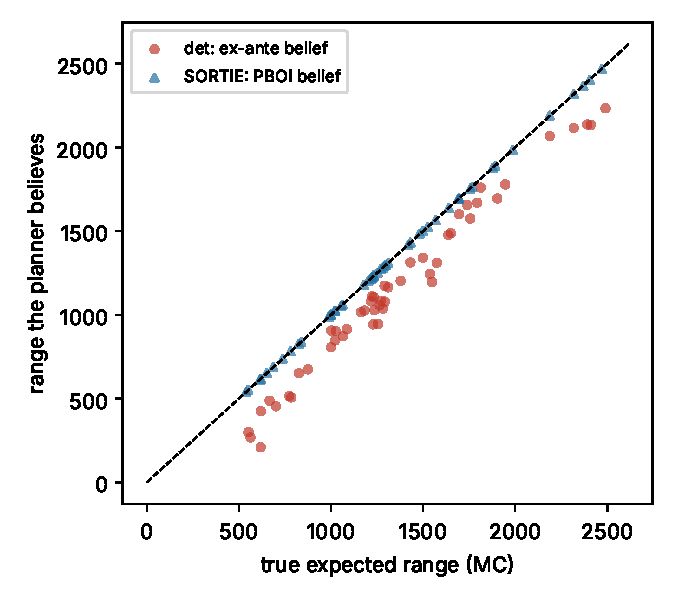
\includegraphics[width=0.48\textwidth]{illusion_range.pdf}\hfill
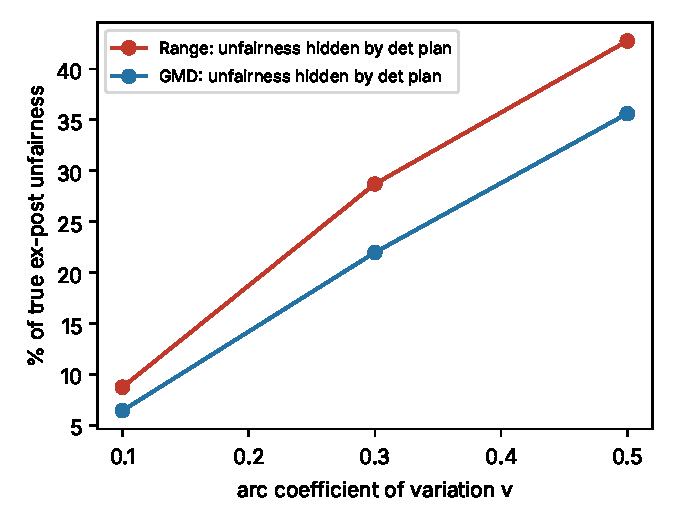
\includegraphics[width=0.48\textwidth]{e6_illusion_v.pdf}
\caption{Left: range believed by Det (ex-ante) and by SORTIE (PBOI) against
the true expected range, E3. Right: share of the true ex-post unfairness that
a deterministic plan does not see, against $v$ (E6).}\label{fig:illusion}
\end{figure}

\subsection{Larger instances (E7, E7b)}
E7 runs $n\in\{50,75,100\}$ on six blocks each, with a 120\,s limit, for the
range, GMD and maximum (18 instance--measure pairs per size). With the
screening lower level the search runs about 9000 iterations per run at
$n=50$ and 3500 at $n=100$ for SORTIE-0 (Det: 15\,000 and 4400). PBOI remains
accurate (mean absolute error $0.15\%$, at most $0.9\%$) and the deterministic
belief error is $-17\%$ on average, as on the small instances.

Table~\ref{tab:e7} pools the 18 pairs per size. SORTIE-0 improves on Det by
about $2\%$ at every size and is better on 12--13 of 18 pairs; the improvement
is significant at $n=50$ ($p=0.035$) but not at $n=75$ or $n=100$
($p=0.17$). SORTIE-1 is significant at $n=50$ but not beyond: its lower level
runs a dichotomic search per route and completes only about 850 iterations at
$n=100$, and $56\%$ of its runs there ($39\%$ at $n=75$) still improved by
more than $0.5\%$ in the second half of the time limit. Single runs at $n\ge75$ are thus dominated by search
noise, especially for the range and the GMD, whose value depends on a few
routes.

E7b separates the method from the search noise at $n=100$: the six instances
and three measures are solved by Det, SAA and SORTIE-0 with three solver seeds
each and a 240\,s limit, and each method is represented by the mean ex-post
value over its seeds (Table~\ref{tab:e7b}). Averaged over seeds, SORTIE-0
improves on Det by $4.2\%$ (median $2.5\%$, better on 13 of 18 pairs,
$p=0.021$); SAA improves by $3.2\%$ ($p=0.10$). The difference between
SORTIE-0 and SAA ($1.1\%$, 12 of 18) is not significant ($p=0.25$), and no
single measure is significant on six instances. The seed-to-seed variation is
itself informative: for the range, the ex-post value of the Det plan varies by
$11\%$ across seeds, that of SORTIE-0 by $3\%$. The deterministic range is flat
over many plans whose realised fairness differs, and the search picks among
them arbitrarily; the ex-post objective distinguishes them. Even at 240\,s,
19\% of the SORTIE-0 runs improved their in-model value by more than
$0.5\%$ in the second half of the run, so the absolute values at $n=100$ are
not fully converged.

\begin{table}[t]\centering\small
\caption{E7: improvement of the ex-post value over Det, $B=1.10$, 120\,s,
pooled over six instances and three measures (range, GMD, max); format as
Table~\ref{tab:e3}.}\label{tab:e7}
\begin{tabular}{lrrr}\toprule
$n$ & SAA & SORTIE-0 & SORTIE-1 \\
\midrule
50 & +1.56 (12/18) & +2.04$^\ast$ (13/18) & +1.20$^\ast$ (15/18) \\
75 & +1.96 (11/18) & +2.04 (13/18) & -0.29 (11/18) \\
100 & +1.52 (10/18) & +2.21 (12/18) & -0.04 (8/18) \\
\bottomrule
\end{tabular}

\end{table}

\begin{table}[t]\centering\small
\caption{E7b, $n=100$, $B=1.10$, 240\,s, three solver seeds: improvement of
the seed-averaged ex-post value over Det (six instances per measure; format as
Table~\ref{tab:e3}) and coefficient of variation of the ex-post value across
seeds, averaged over instances.}\label{tab:e7b}
\begin{tabular}{lrrrrr}\toprule
 & \multicolumn{2}{c}{vs Det, mean of 3 seeds} & \multicolumn{3}{c}{Seed CV (\%)} \\
Measure & SAA & SORTIE-0 & Det & SAA & SORTIE-0 \\
\midrule
Range & +6.45 (4/6) & +8.68 (5/6) & 11.3 & 4.7 & 3.0 \\
GMD & +2.49 (3/6) & +3.18 (4/6) & 6.4 & 2.7 & 4.5 \\
Max & +0.78 (4/6) & +0.86 (4/6) & 1.4 & 0.8 & 1.4 \\
\midrule
All & +3.24 (11/18) & +4.24$^\ast$ (13/18) & \multicolumn{3}{l}{SORTIE-0 vs SAA: +1.09 (12/18)} \\
\bottomrule
\end{tabular}

\end{table}

Figure~\ref{fig:convergence} shows the anytime behaviour behind these
numbers, and Figure~\ref{fig:seeds} the seed-to-seed spread at $n=100$.

\begin{figure}[t]\centering
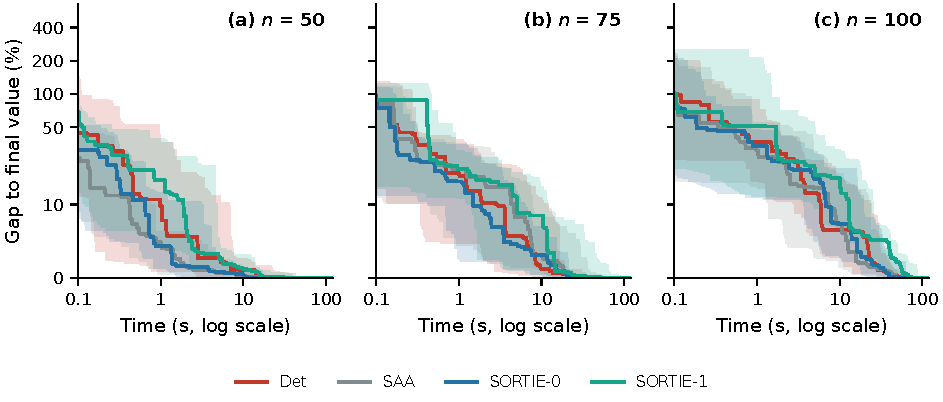
\includegraphics[width=\textwidth]{fig_convergence.pdf}
\caption{E7: best in-model value relative to the final value over the run
(median and interquartile range over the 18 runs per method and size).}\label{fig:convergence}
\end{figure}

\begin{figure}[t]\centering
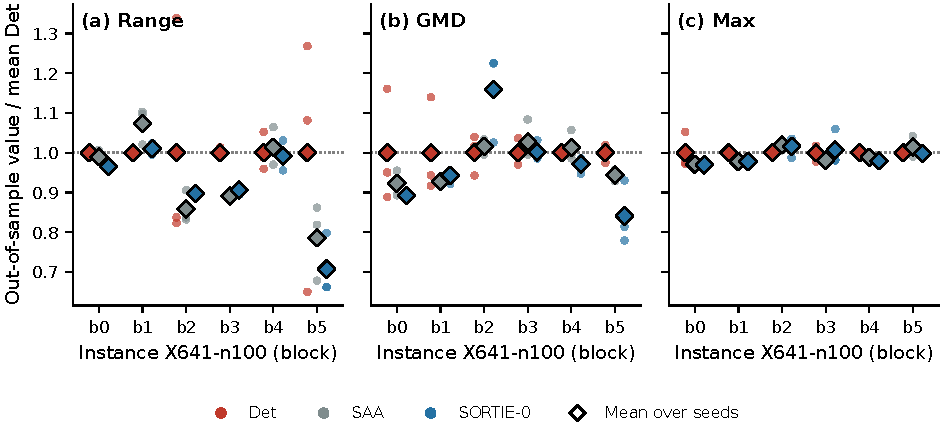
\includegraphics[width=\textwidth]{fig_e7b_seeds.pdf}
\caption{E7b, $n=100$: ex-post value of each solver seed, relative to the mean
Det value of the instance; larger markers: seed means.}\label{fig:seeds}
\end{figure}

\subsection{Heterogeneous noise: congestion (E8)}
E3 suggests that the stochastic refinement matters little when a route's
variance is proportional to its length. E8 breaks that proportionality: arcs
near a congestion centre have up to twice the base coefficient of variation
and arcs far from it a third. We rerun the main grid ($B=1.10$; range, GMD
and max) on the congested versions of the same 25 instances, starting from
the same cost plans.

The illusion becomes somewhat larger: a deterministic plan understates its
range by $26\%$, its GMD by $22\%$ and its maximum by $10\%$, against $23\%$,
$19\%$ and $9\%$ on the same cells under homogeneous noise. The PBOI belief
has a mean signed error below $0.2\%$ (mean absolute error at most
$0.26\%$).
The gain of optimising ex-post fairness, however, grows only slightly
(Table~\ref{tab:e8}). Pooled over 75 runs, SORTIE-0 improves on Det by
$1.51\%$ (median $1.24\%$; better in 53, worse in 3; $p<10^{-8}$) and
SORTIE-1 by $1.66\%$ (better in 57, worse in 10), against $1.36\%$ for
SORTIE-0 on the same cells without congestion. By measure the change is
$0.94\%\to1.40\%$ for the GMD, $2.08\%\to2.15\%$ for the maximum and
$1.07\%\to0.96\%$ for the range. SAA gains $1.28\%$, but with a median of only
$0.47\%$, and SORTIE-0 beats it head to head in 49 of 75 runs (worse in 6;
$p<10^{-6}$). The CVaR$_{0.9}$ of the range is 1919 for Det, 1905 for SAA,
1912 for SORTIE-0 and 1907 for SORTIE-1. Heterogeneous noise thus makes a
deterministic plan's self-assessment much worse, but in our instances it
changes the best plan only a little more than homogeneous noise does: the
congested arcs are concentrated in one part of the network, and the
assignment that balances lengths still roughly balances risk there.

\begin{table}[t]\centering\small
\caption{E8: congested arc noise, $B=1.10$, 25 instances per row;
improvement of the ex-post value over Det (format as Table~\ref{tab:e3}).}\label{tab:e8}
\begin{tabular}{lrrr}\toprule
Measure & SAA & SORTIE-0 & SORTIE-1 \\
\midrule
GMD & +0.76 (11/25) & +1.40$^\ast$ (13/25) & +1.82$^\ast$ (15/25) \\
Max & +1.87$^\ast$ (23/25) & +2.15$^\ast$ (23/25) & +2.21$^\ast$ (24/25) \\
Range & +1.22 (13/25) & +0.96$^\ast$ (17/25) & +0.94$^\ast$ (18/25) \\
\bottomrule
\end{tabular}

\end{table}


%==========================================================================
Figure~\ref{fig:congestion} shows the congestion multiplier on the
illustrative instance, and Figure~\ref{fig:e8e3} pairs every instance and
measure with and without congestion: the points scatter around the diagonal,
with the GMD above it and the range on both sides.

\begin{figure}[t]\centering
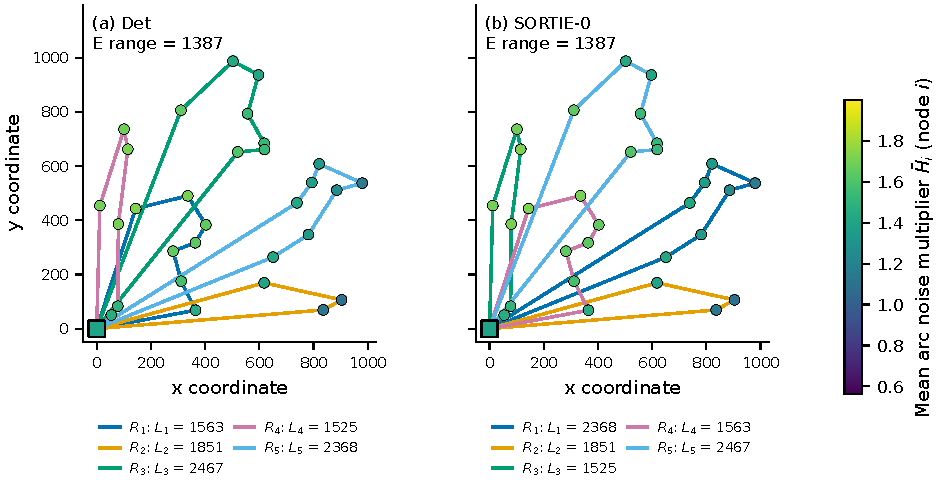
\includegraphics[width=\textwidth]{fig_congestion.pdf}
\caption{X641-n30-b0 with congestion: customers coloured by the mean noise
multiplier $H$ of their arcs, with the range-optimised Det and SORTIE-0 plans of E8.}\label{fig:congestion}
\end{figure}

\begin{figure}[t]\centering
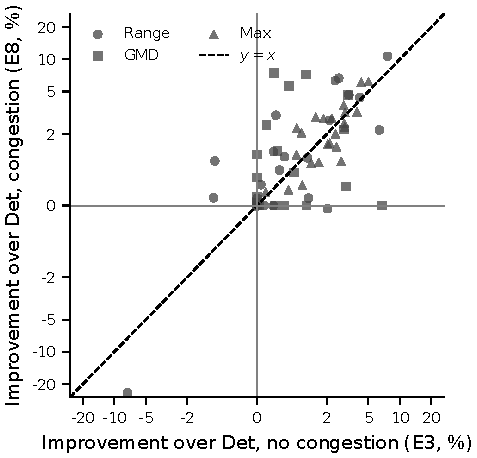
\includegraphics[width=0.6\textwidth]{fig_e8_vs_e3.pdf}
\caption{Improvement of SORTIE-0 over Det per instance and measure, without
(E3) and with (E8) congestion, $B=1.10$.}\label{fig:e8e3}
\end{figure}

\subsection{The budget frontier (E9)}
E9 repeats the comparison of Det and SORTIE-0 on the 10 instances with
$n\in\{25,35\}$ for budget factors $B$ from $1.02$ to $1.30$
(Table~\ref{tab:e9}, Figure~\ref{fig:frontier}). Two effects stand out. First,
the gain of SORTIE-0 grows with the budget: from about $1\%$ for $B\le1.10$ to
$3.2\%$ at $B=1.15$ and $6.8\%$ at $B=1.30$, where SORTIE-0 is better on all 30
instance--measure pairs. With little slack every fair plan is close to the
cost-optimal one and there is little room to choose; with more slack there
are many plans whose deterministic range is about equal but whose realised
range differs, and only the ex-post objective can tell them apart. Second,
for $B\ge1.15$ SORTIE-0 uses \emph{less} of the budget (below that the total
lengths agree within $0.3$ percentage points). At $B=1.30$ the Det plans for the
maximum have a total length $20.5\%$ above $C^\ast$ and an expected realised
maximum $5.2\%$ below that of the cost plan; the SORTIE-0 plans use $13.5\%$
and achieve $8.7\%$. For the maximum the deterministic objective even
deteriorates from $B=1.20$ to $B=1.30$: the extra length it buys goes into
routes whose deterministic length is irrelevant to the maximum but whose
variance raises the realised one. At every budget level the ex-post objective reaches lower realised
unfairness, and for generous budgets it does so with less total length.

The same cells at $B=1.10$ appear in E3, and the per-cell means differ (for
example $-0.7\%$ for the range in E9 against $+0.9\%$ in E3 on the
same ten instances). The runs are identical except for wall-clock
timing: the search stops at a time limit, so the iteration at which it stops,
and hence the plan, can differ between two executions on a shared machine.
This is another manifestation of the search noise analysed in E7b, and the
reason we draw conclusions only from pooled comparisons.

\begin{table}[t]\centering\small
\caption{E9: improvement of the ex-post value of SORTIE-0 over Det by budget
factor, $n\in\{25,35\}$, ten instances per measure; cost ratio: mean
$\sum_kL_k/C^\ast$ of the SORTIE-0 plans (format as Table~\ref{tab:e3}).}\label{tab:e9}
\begin{tabular}{lrcccc}
\toprule
$B$ & Cost ratio & Pooled & Range & GMD & Max \\
\midrule
1.02 & 1.014 & +1.43$^\ast$ (17/30) & +1.40 (4/10) & +2.07 (5/10) & +0.82$^\ast$ (8/10) \\
1.05 & 1.041 & +0.73$^\ast$ (19/30) & +0.81 (5/10) & +0.66 (5/10) & +0.73$^\ast$ (9/10) \\
1.10 & 1.094 & +0.67$^\ast$ (20/30) & -0.72 (7/10) & +0.30 (3/10) & +2.45$^\ast$ (10/10) \\
1.15 & 1.134 & +3.20$^\ast$ (27/30) & +5.92$^\ast$ (8/10) & +1.31 (9/10) & +2.37$^\ast$ (10/10) \\
1.20 & 1.170 & +2.46$^\ast$ (26/30) & +2.59 (9/10) & +2.34$^\ast$ (7/10) & +2.46$^\ast$ (10/10) \\
1.30 & 1.222 & +6.79$^\ast$ (30/30) & +7.64$^\ast$ (10/10) & +9.11$^\ast$ (10/10) & +3.63$^\ast$ (10/10) \\
\bottomrule
\end{tabular}

\end{table}

\begin{figure}[t]\centering
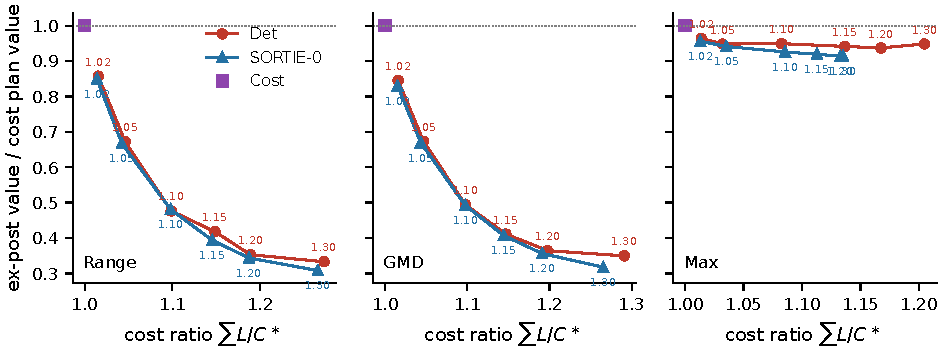
\includegraphics[width=\textwidth]{fig_e9_frontier.pdf}
\caption{E9: price of fairness. Mean total length relative to $C^\ast$
against the mean expected realised unfairness relative to the cost-optimal
plan, for budget factors $B$ from 1.02 to 1.30 (labels).}\label{fig:frontier}
\end{figure}

\subsection{Fleet size (E10)}
E10 varies the number of vehicles on the $n=35$ instances, with capacity
$\lfloor\sum_iq_i/(m-1)\rfloor$ so that one vehicle's worth of slack remains
(Table~\ref{tab:e10}, Figure~\ref{fig:e10}). The illusion grows with $m$:
a deterministic plan understates its range by $10\%$ with three vehicles,
$24\%$ with five and $27\%$ with seven. More routes compete for the extreme
ranks, so more of the realised unfairness comes from which route happens to
be longest on the day, which a deterministic model cannot see. The gain of
SORTIE-0 is small with three and five vehicles ($0.5\%$ and $0.6\%$; with
$m=5$ not significant on these 15 pairs, $p=0.06$) and $3.2\%$ with seven
(better on 13 of 15 pairs, $p=0.001$). With $m=3$ the GMD is
proportional to the range ($4/9$ of it), so the two rows coincide.

\begin{table}[t]\centering\small
\caption{E10: fleet size, $n=35$, five instances per measure, $B=1.10$
(format as Table~\ref{tab:e3}).}\label{tab:e10}
\begin{tabular}{llrcc}
\toprule
$m$ & Measure & Det belief err. (\%) & SAA vs Det & SORTIE-0 vs Det \\
\midrule
3 & Pooled & -8.2 & +2.83$^\ast$ (7/15) & +0.48$^\ast$ (8/15) \\
3 & Range & -9.9 & +3.66 (2/5) & +0.14 (2/5) \\
3 & GMD & -9.9 & +3.66 (2/5) & +0.14 (2/5) \\
3 & Max & -4.6 & +1.17 (3/5) & +1.17 (4/5) \\
5 & Pooled & -18.6 & -1.62 (8/15) & +0.64 (9/15) \\
5 & Range & -24.1 & -3.11 (2/5) & +2.78 (3/5) \\
5 & GMD & -23.2 & -4.01 (1/5) & -3.58 (1/5) \\
5 & Max & -8.5 & +2.26 (5/5) & +2.71 (5/5) \\
7 & Pooled & -20.3 & +2.34$^\ast$ (10/15) & +3.16$^\ast$ (13/15) \\
7 & Range & -26.7 & +1.36 (3/5) & +4.58 (5/5) \\
7 & GMD & -23.3 & +3.34 (2/5) & +2.14 (3/5) \\
7 & Max & -10.9 & +2.31 (5/5) & +2.76 (5/5) \\
\bottomrule
\end{tabular}

\end{table}

\begin{figure}[t]\centering
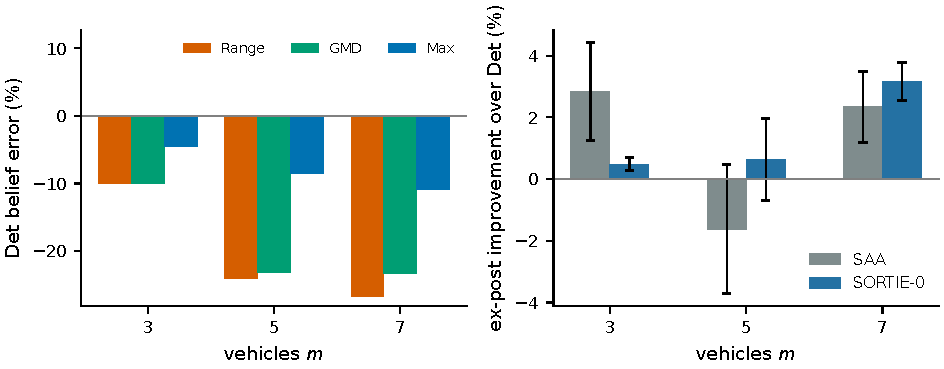
\includegraphics[width=\textwidth]{fig_e10.pdf}
\caption{E10: belief error of Det and improvement over Det against the
number of vehicles.}\label{fig:e10}
\end{figure}

\subsection{Common shocks in practice (E11)}
E11 re-evaluates all 500 E3 plans with $B=1.10$ under day-factor
dispersions $s_Y\in\{0,0.15,0.3,0.5\}$, using the same arc draws
(Table~\ref{tab:e11}, Figure~\ref{fig:e11}). As Proposition~3
predicts, the expected ordered measures are unchanged: the ratio of the value
with and without the day factor is $1.000$ up to Monte Carlo error (at most
$1.0007$ on average, at $s_Y=0.5$). The expected empirical variance is
multiplied by $1.023$, $1.095$ and $1.285$, against $e^{s_Y^2}=1.023$, $1.094$
and $1.284$. The tail is a different matter: the CVaR$_{0.9}$ of the realised
range grows by $7\%$, $25\%$ and $58\%$. A fleet-wide shock is irrelevant for
the choice of a plan by expected ordered fairness, but not for the risk of a
very unfair day.

\begin{table}[t]\centering\small
\caption{E11: ratio of each measure with the day factor to its value without,
mean $\pm$ standard deviation over the 500 E3 plans with $B=1.10$.}\label{tab:e11}
\resizebox{\textwidth}{!}{\begin{tabular}{lccccccc}
\toprule
$s_Y$ & Max & Range & GMD & MAD & Var & CVaR90 range & $e^{s_Y^2}$ \\
\midrule
0.00 & 1.000 $\pm$ 0.000 & 1.000 $\pm$ 0.000 & 1.000 $\pm$ 0.000 & 1.000 $\pm$ 0.000 & 1.000 $\pm$ 0.000 & 1.000 $\pm$ 0.000 & 1.000 \\
0.15 & 1.000 $\pm$ 0.001 & 1.000 $\pm$ 0.001 & 1.000 $\pm$ 0.001 & 1.000 $\pm$ 0.001 & 1.023 $\pm$ 0.002 & 1.074 $\pm$ 0.016 & 1.023 \\
0.30 & 1.000 $\pm$ 0.002 & 1.000 $\pm$ 0.002 & 1.000 $\pm$ 0.002 & 1.000 $\pm$ 0.002 & 1.095 $\pm$ 0.005 & 1.251 $\pm$ 0.042 & 1.094 \\
0.50 & 1.001 $\pm$ 0.003 & 1.001 $\pm$ 0.003 & 1.001 $\pm$ 0.003 & 1.001 $\pm$ 0.003 & 1.285 $\pm$ 0.011 & 1.579 $\pm$ 0.081 & 1.284 \\
\bottomrule
\end{tabular}
}
\end{table}

\begin{figure}[t]\centering
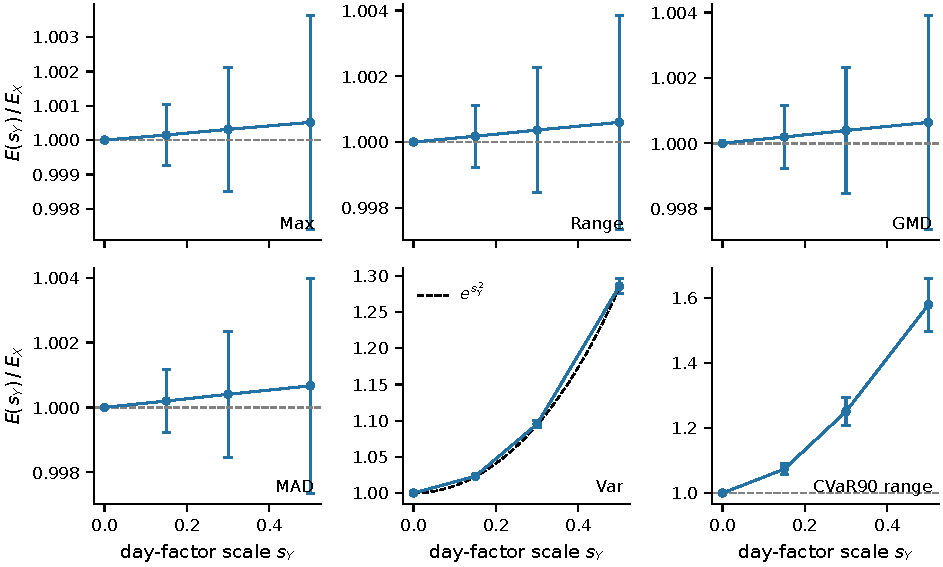
\includegraphics[width=\textwidth]{fig_e11.pdf}
\caption{E11: effect of the day-factor dispersion $s_Y$ on the expected
ordered measures, the expected variance and the CVaR of the range.}\label{fig:e11}
\end{figure}


\subsection{Robustness to the noise model (E12)}
PBOI assumes independent route durations with given means and variances,
and SORTIE was tuned to gamma arc noise. E12 re-evaluates the $B=1.10$ plans
of E3 (500 plans) under four arc-noise families, and those of E8 (300 plans)
under the first two (the other two cannot reach the low per-arc variability
of the uncongested arcs of E8) with the
same mean and coefficient of variation per arc: gamma (the planning model),
lognormal (heavier right tail), \emph{incident} (with probability $0.02$ an
arc takes $2.5$ times as long, the rest of the variability being gamma), and
\emph{regional} (a multiplicative factor shared by all arcs whose tail lies in
the same quadrant of the plane, which makes routes in the same region
positively correlated and so violates the independence that PBOI assumes)
(Table~\ref{tab:e12}, Figure~\ref{fig:e12}).

The accuracy of PBOI degrades gracefully. Under lognormal noise its mean
absolute error rises from $0.16\%$ to $0.29\%$; under incidents to $1.4\%$, with
a bias of $+1.4\%$ (it overstates unfairness) and a worst case of $9.5\%$; under regional correlation to $1.9\%$, with a
worst case of $20\%$ for the variance measure, the one most affected by
correlation. What matters for planning is that the ranking of plans survives:
under every family SORTIE-0 remains significantly better than Det, by $1.0\%$
to $1.2\%$ on the E3 plans and $1.5\%$ on the E8 plans (gamma and lognormal), against $1.2\%$ and
$1.5\%$ under the planning model.

\begin{table}[t]\centering\small
\caption{E12: noise-model misspecification. PBOI error of the gamma-based
prediction against the true expected value under each family, and
improvement of SORTIE-0 over Det evaluated under that family (format as
Table~\ref{tab:e3}).}\label{tab:e12}
\resizebox{\textwidth}{!}{\begin{tabular}{llrrrc}
\toprule
Family & Source & Plans & PBOI $|$err$|$ (\%) & PBOI signed err. (\%) & SORTIE-0 vs Det \\
\midrule
Gamma & E3 & 500 & 0.16 & +0.04 & +1.23$^\ast$ (81/125) \\
Incident & E3 & 500 & 1.43 & +1.35 & +1.03$^\ast$ (71/125) \\
Lognormal & E3 & 500 & 0.29 & +0.16 & +1.21$^\ast$ (82/125) \\
Regional & E3 & 500 & 1.88 & -0.74 & +0.96$^\ast$ (65/125) \\
Gamma & E8 & 300 & 0.18 & +0.10 & +1.51$^\ast$ (53/75) \\
Lognormal & E8 & 300 & 0.51 & +0.40 & +1.48$^\ast$ (55/75) \\
\bottomrule
\end{tabular}
}
\end{table}

\begin{figure}[t]\centering
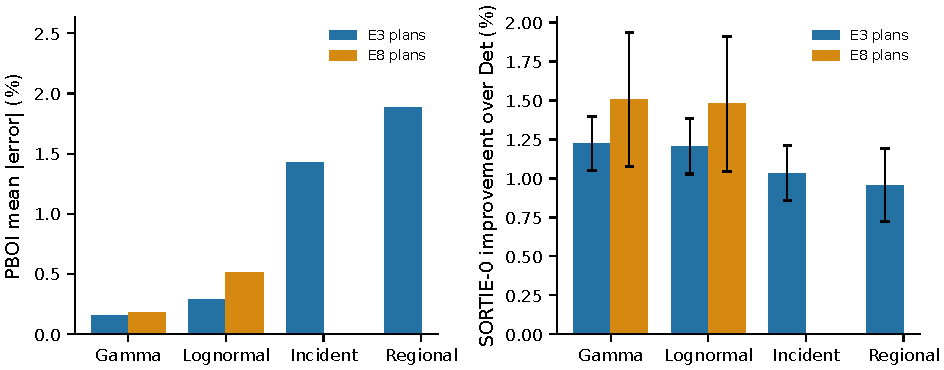
\includegraphics[width=\textwidth]{fig_e12.pdf}
\caption{E12: PBOI error and improvement of SORTIE-0 over Det under four
arc-noise families.}\label{fig:e12}
\end{figure}


\subsection{Risk attitude of the drivers (E13)}
E13 solves the $n\in\{25,35\}$ instances with the risk-consistent lower level
for $\kappa\in\{0,0.5,1,2,4\}$ (Table~\ref{tab:e13}, Figure~\ref{fig:e13}).
Under homogeneous noise the risk-consistent tour rarely differs from the
shortest one: even at $\kappa=4$ only $14$--$16\%$ of the routes change, and
the extra length is about 13 distance units per plan, under $0.2\%$ of the
total. The ex-post value changes by less than the search noise (median ratio
to $\kappa=0$ equal to one, interquartile range within $\pm1\%$). The reason is
that, for a fixed customer set, a tour's length and its quadratic length are
nearly comonotone: the shortest tour is also nearly the least variable one.
Proposition~11 shows that this need not be so, and with
heterogeneous noise the two can separate, but on these instances the choice of
$\kappa$ is a matter of the drivers' preferences rather than of fairness.

\begin{table}[t]\centering\small
\caption{E13: risk-consistent lower level, $n\in\{25,35\}$, $B=1.10$, ten
instances per row. Routes changed: share of routes whose tour differs from
the shortest tour of the same customers; extra length: total, per plan; mean
risk: mean of $L_k+v\sqrt{W_k}$.}\label{tab:e13}
\resizebox{\textwidth}{!}{\begin{tabular}{llrrrrr}
\toprule
Measure & $\kappa$ & Routes changed (\%) & Extra length & Mean risk & Ex-post vs $\kappa{=}0$ [IQR] & Cost ratio \\
\midrule
Range & 0 & 0.0 & 0.0 & 1913.9 & 1.000 [1.000, 1.000] & 1.098 \\
Range & 0.5 & 6.0 & 1.0 & 1912.9 & 1.000 [0.998, 1.000] & 1.098 \\
Range & 1 & 4.0 & 0.9 & 1915.6 & 1.000 [0.995, 1.000] & 1.098 \\
Range & 2 & 14.0 & 9.2 & 1914.0 & 1.000 [0.989, 1.004] & 1.099 \\
Range & 4 & 14.0 & 14.1 & 1911.4 & 0.997 [0.989, 1.004] & 1.099 \\
Max & 0 & 0.0 & 0.0 & 1890.7 & 1.000 [1.000, 1.000] & 1.086 \\
Max & 0.5 & 2.0 & 0.5 & 1885.9 & 1.000 [1.000, 1.000] & 1.084 \\
Max & 1 & 6.0 & 2.6 & 1891.3 & 1.000 [1.000, 1.000] & 1.087 \\
Max & 2 & 6.0 & 3.9 & 1887.0 & 1.000 [1.000, 1.000] & 1.085 \\
Max & 4 & 16.0 & 12.4 & 1882.6 & 1.000 [1.000, 1.000] & 1.083 \\
\bottomrule
\end{tabular}
}
\end{table}

\begin{figure}[t]\centering
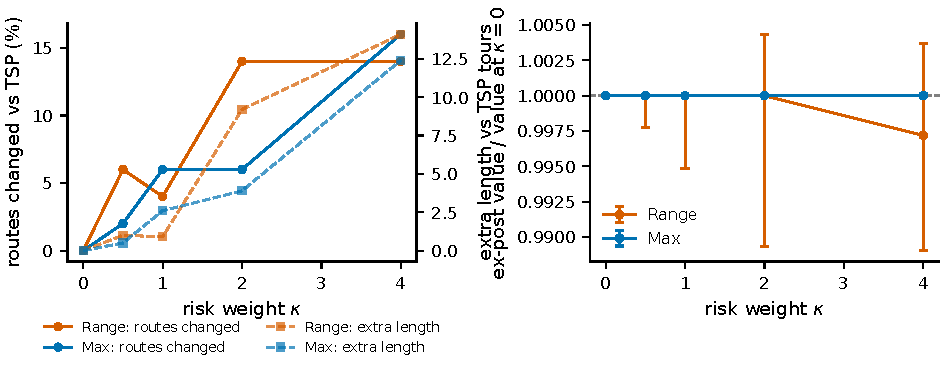
\includegraphics[width=\textwidth]{fig_e13.pdf}
\caption{E13: effect of the drivers' risk weight $\kappa$.}\label{fig:e13}
\end{figure}

\subsection{Why the rank prices work (E14)}
E14 checks the first-order model behind the screen directly. For the
cost-optimal start plan and the final SORTIE-0 plan of the ten
$n\in\{25,35\}$ instances, we evaluated up to 400 relocate and swap moves
both by the rank-price prediction and exactly (exact lower level and PBOI);
5577 moves in total (Table~\ref{tab:e14}, Figures~\ref{fig:e14scatter}
and~\ref{fig:e14topk}). The prediction ranks the moves almost as the exact
evaluation does: Spearman's $\rho$ is $0.89$--$0.94$ on the start plans and
$0.78$--$0.89$ on the final plans. On the start plans the exact-best improving
move is among the 8 best predicted moves in $80\%$ of the cases (random
ordering: $7\%$) and always among the 21 best. On the final plans of SORTIE-0
there is no improving relocate or swap move in 28 of 30 cases: the search
ends in genuine local optima of its neighbourhood. Consistently, the number of
candidates $K$ evaluated per step barely matters (Table~\ref{tab:e14k}): the
median ex-post value is the same for $K$ from 1 to 32.

\begin{table}[t]\centering\small
\caption{E14: rank-price prediction against exact evaluation. Groups:
(instance, plan) pairs with at least one exactly improving move; top-8 hit:
share of those groups in which the exact-best improving move is among the 8
best predicted moves (in brackets: expected share under a random order).}\label{tab:e14}
\resizebox{\textwidth}{!}{\begin{tabular}{llrrrc}
\toprule
Measure & Plans & Moves & Groups with improving move & Spearman $\rho$ & Top-8 hit (random) \\
\midrule
Range & Cost plan & 1448 & 10/10 & 0.93 & 0.80 (0.07) \\
Range & SORTIE-0 plan & 346 & 1/10 & 0.80 & 0.00 (0.19) \\
Range & All plans & 1794 & 11/20 & 0.92 & 0.73 (0.08) \\
GMD & Cost plan & 1448 & 10/10 & 0.94 & 0.80 (0.07) \\
GMD & SORTIE-0 plan & 333 & 0/10 & 0.78 & -- (--) \\
GMD & All plans & 1781 & 10/20 & 0.94 & 0.80 (0.07) \\
Max & Cost plan & 1448 & 10/10 & 0.89 & 0.80 (0.07) \\
Max & SORTIE-0 plan & 554 & 1/10 & 0.89 & 0.00 (0.21) \\
Max & All plans & 2002 & 11/20 & 0.89 & 0.73 (0.08) \\
\bottomrule
\end{tabular}
}
\end{table}

\begin{table}[t]\centering\small
\caption{E14: number of candidates $K$ evaluated per step; ex-post value
relative to $K=8$, median and interquartile range over 20 instance--measure
pairs.}\label{tab:e14k}
\begin{tabular}{rcc}
\toprule
$K$ & Range median [IQR] & GMD median [IQR] \\
\midrule
1 & 1.000 [1.000, 1.000] & 1.000 [1.000, 1.000] \\
2 & 1.000 [1.000, 1.000] & 1.000 [1.000, 1.000] \\
4 & 1.000 [1.000, 1.000] & 1.000 [1.000, 1.000] \\
8 & 1.000 [1.000, 1.000] & 1.000 [1.000, 1.000] \\
16 & 1.000 [1.000, 1.000] & 1.000 [0.996, 1.000] \\
32 & 1.000 [0.994, 1.000] & 1.000 [1.000, 1.000] \\
\bottomrule
\end{tabular}

\end{table}

\begin{figure}[t]\centering
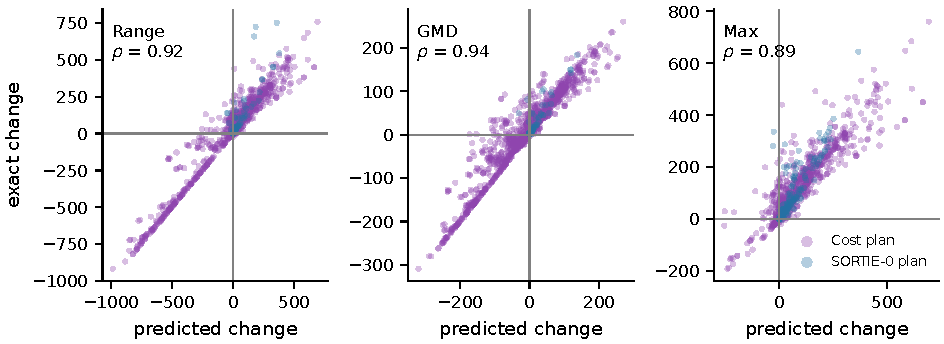
\includegraphics[width=\textwidth]{fig_e14_scatter.pdf}
\caption{E14: predicted (rank prices) against exact change of the
objective for 5577 moves.}\label{fig:e14scatter}
\end{figure}

\begin{figure}[t]\centering
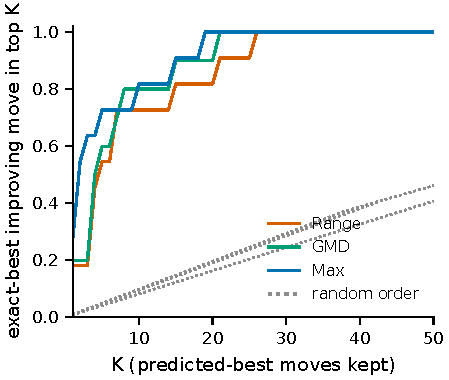
\includegraphics[width=0.55\textwidth]{fig_e14_topk.pdf}
\caption{E14: share of cases in which the exact-best improving move is among
the $K$ best predicted moves.}\label{fig:e14topk}
\end{figure}

\subsection{Is a larger sample enough? (E15)}
A natural objection is that SAA with 200 scenarios is simply too small. E15
reruns SAA with $S\in\{50,200,1000,5000\}$ scenarios on the $n\in\{25,35\}$
instances (Table~\ref{tab:e15}, Figure~\ref{fig:e15}). SORTIE-0 is better than every
SAA variant on average: by $1.4\%$ ($S=50$), $1.6\%$ ($S=200$), $1.1\%$
($S=1000$) and $0.9\%$ ($S=5000$), significantly for $S\le1000$. The gap shrinks as the sample grows, as it should, since
SAA converges to the objective that PBOI evaluates exactly; with 5000
scenarios SAA is still worse on 9 pairs and better on 2 (the rest tied), but
the difference is no longer significant at the $5\%$ level ($p=0.0505$). The sample average is cached per route, so the number of iterations
drops only from about 5300 to 4200, and the remaining gap is the sampling
error of the objective, not a lack of search time.

\begin{table}[t]\centering\small
\caption{E15: improvement of SORTIE-0 over SAA with $S$ scenarios, $n\in\{25,35\}$,
$B=1.10$, ten instances per measure (format as Table~\ref{tab:e3}; positive:
SORTIE-0 better).}\label{tab:e15}
\begin{tabular}{rccccc}
\toprule
$S$ & Range & GMD & Max & Pooled & $p$ (pooled) \\
\midrule
50 & +0.17 (6/10) & +2.88$^\ast$ (8/10) & +0.99$^\ast$ (8/10) & +1.35$^\ast$ (22/30) & 0.001 \\
200 & +2.11$^\ast$ (7/10) & +2.15$^\ast$ (7/10) & +0.46$^\ast$ (10/10) & +1.57$^\ast$ (24/30) & 0.000 \\
1000 & +1.45 (5/10) & +1.64 (4/10) & +0.19 (6/10) & +1.09$^\ast$ (15/30) & 0.002 \\
5000 & +1.34 (3/10) & +1.38 (2/10) & +0.02 (4/10) & +0.91 (9/30) & 0.050 \\
\bottomrule
\end{tabular}

\end{table}

\begin{figure}[t]\centering
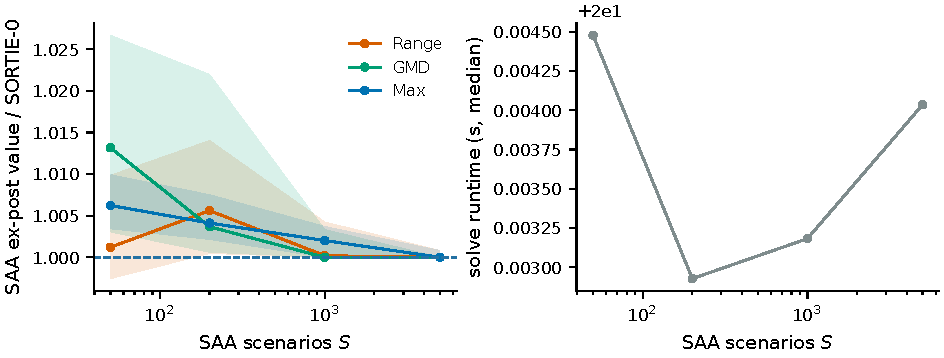
\includegraphics[width=\textwidth]{fig_e15.pdf}
\caption{E15: ex-post value of SAA relative to SORTIE-0 against the sample
size $S$.}\label{fig:e15}
\end{figure}

\subsection{Simpler stochastic baselines (E16)}
Two simpler ways of taking uncertainty into account are tested on the full E3
grid at $B=1.10$ (Table~\ref{tab:e16}). \emph{Det-$\sigma$} applies the
deterministic ordered measure to risk-adjusted lengths $L_k+\sigma_k$, the
fairness analogue of the robust-length heuristics common in stochastic
routing. It is \emph{worse} than Det ($-0.8\%$, better on 37 and worse on 61 of
125 pairs, $p=0.02$), and SORTIE-0 beats it by $1.9\%$ (97 of 125, $p<10^{-14}$).
Adding a standard deviation to every route treats each route's risk
separately, whereas the expected ordered measure depends on how likely each
route is to occupy each rank, which is what the Poisson--binomial integral
and the rank prices capture. \emph{PBOI-N} replaces the gamma marginals by
normal ones; it performs like SORTIE-0 (no significant difference, $p=0.65$),
so the method is insensitive to the marginal family once the first two
moments are right.

\begin{table}[t]\centering\small
\caption{E16: risk-adjusted deterministic (Det-$\sigma$) and normal-marginal
(PBOI-N) objectives, E3 grid, $B=1.10$ (format as Table~\ref{tab:e3}; the
variance is omitted for PBOI-N because the expected empirical variance does
not depend on the marginal family).}\label{tab:e16}
\begin{tabular}{lcccc}
\toprule
Measure & Det-$\sigma$ vs Det & PBOI-N vs Det & SORTIE-0 vs Det & SORTIE-0 vs Det-$\sigma$ \\
\midrule
Range & -0.49 (8/25) & +0.48$^\ast$ (18/25) & +1.07$^\ast$ (17/25) & +1.51$^\ast$ (19/25) \\
GMD & -0.69 (8/25) & +0.83$^\ast$ (14/25) & +0.94$^\ast$ (14/25) & +1.50$^\ast$ (18/25) \\
Max & -0.08 (8/25) & +2.08$^\ast$ (24/25) & +2.08$^\ast$ (24/25) & +2.13$^\ast$ (25/25) \\
Pooled & -0.81$^\dagger$ (37/125) & +1.10$^\ast$ (71/100) & +1.23$^\ast$ (81/125) & +1.86$^\ast$ (97/125) \\
\bottomrule
\end{tabular}

\end{table}

\subsection{A second benchmark family (E17)}\label{sec:e17}
All instances so far are slices of one file, and slicing places the depot at
the first node of each block. E17 tests twelve further CVRPLIB X instances of
\citet{uchoa2017new} (X-n101-k25 to X-n153-k22), which were generated with
different depot positions and customer distributions. From each we take the depot of the file and its
first 50 customers, keep $m=5$ and the capacity rule $Q=\lfloor\sum_iq_i/4\rfloor$,
and solve range, GMD and maximum at $B=1.10$ with Det, SAA, SORTIE-0 and
Det-$\sigma$, 120\,s and two solver seeds; each method is represented by the
mean ex-post value over its seeds (Tables~\ref{tab:e17}
and~\ref{tab:e17inst}, Figure~\ref{fig:e17}).

The results are stronger than on the sliced instances. The illusion reaches
$40\%$ for the range and $35\%$ for the GMD, against $23\%$ and $19\%$ on the
sliced instances at the same budget; plausibly the file's own depot, which is often eccentric,
makes the routes differ more in variance than a block depot does. SORTIE-0 improves on Det by $2.2\%$ on average
(median $1.7\%$; better on 31 and worse on 5 of 36 pairs, $p<10^{-6}$), with a
positive average on every one of the twelve instances ($0.7\%$ to $4.2\%$).
SAA improves by $0.7\%$, and SORTIE-0 beats it on 33 of 36 pairs
($p<10^{-7}$). Det-$\sigma$ is again worse than Det on average ($-0.8\%$; better on 13 and
worse on 23 pairs, not significant here, $p=0.15$). The
conclusions of E3 and E16 thus carry over to instances with other depot
positions and customer distributions, with larger effects.

\begin{table}[t]\centering\small
\caption{E17: second benchmark family (12 X instances, depot plus first 50
customers), $B=1.10$, 120\,s, mean of two solver seeds; improvement of the
ex-post value over Det (format as Table~\ref{tab:e3}).}\label{tab:e17}
\begin{tabular}{lcccc}
\toprule
Measure & SAA vs Det & SORTIE-0 vs Det & Det-$\sigma$ vs Det & Det belief err. (\%) \\
\midrule
Range & +1.48 (8/12) & +2.91$^\ast$ (11/12) & -0.39 (5/12) & -40.3 \\
GMD & -0.62 (5/12) & +1.64 (8/12) & -2.15$^\dagger$ (1/12) & -34.7 \\
Max & +1.36$^\ast$ (10/12) & +1.93$^\ast$ (12/12) & +0.01 (7/12) & -8.4 \\
Pooled & +0.74$^\ast$ (23/36) & +2.16$^\ast$ (31/36) & -0.84 (13/36) & -27.8 \\
\bottomrule
\end{tabular}

\end{table}

\begin{table}[t]\centering\small
\caption{E17 per instance: depot position, $C^\ast$ and the improvement of
SORTIE-0 over Det pooled over the three measures.}\label{tab:e17inst}
\begin{tabular}{lrrr}
\toprule
Instance & Depot & $C^\ast$ & SORTIE-0 vs Det, mean of measures (wins/3) \\
\midrule
X-n101-k25-h50 & intermediate & 7415 & +2.80 (3/3) \\
X-n106-k14-h50 & eccentric & 9767 & +2.02 (3/3) \\
X-n110-k13-h50 & central & 7194 & +3.65 (3/3) \\
X-n115-k10-h50 & central & 7183 & +2.04 (3/3) \\
X-n120-k6-h50 & eccentric & 9809 & +1.89 (3/3) \\
X-n125-k30-h50 & eccentric & 9842 & +1.58 (3/3) \\
X-n129-k18-h50 & eccentric & 9821 & +1.03 (2/3) \\
X-n134-k13-h50 & eccentric & 4686 & +0.69 (2/3) \\
X-n139-k10-h50 & central & 7253 & +4.24 (3/3) \\
X-n143-k7-h50 & eccentric & 10398 & +2.94 (2/3) \\
X-n148-k46-h50 & intermediate & 7752 & +1.76 (2/3) \\
X-n153-k22-h50 & intermediate & 5786 & +1.27 (2/3) \\
\bottomrule
\end{tabular}

\end{table}

\begin{figure}[t]\centering
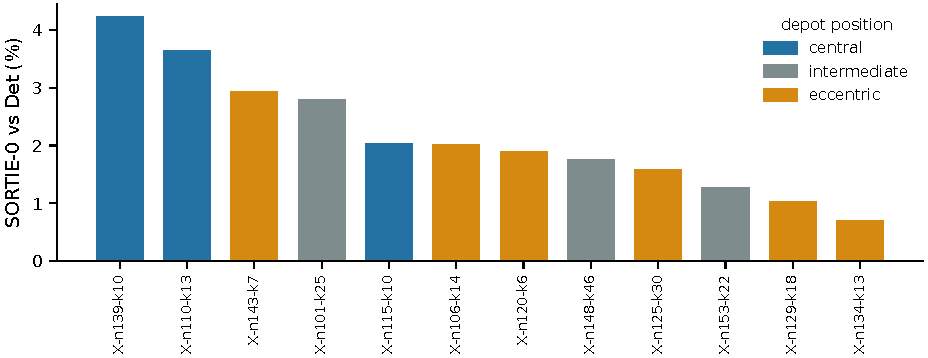
\includegraphics[width=\textwidth]{fig_e17.pdf}
\caption{E17: improvement of SORTIE-0 over Det per instance (mean over
measures and seeds), coloured by depot position.}\label{fig:e17}
\end{figure}



\clearpage
\section{Per-instance results}\label{app:tables}

\begin{figure}[h]\centering
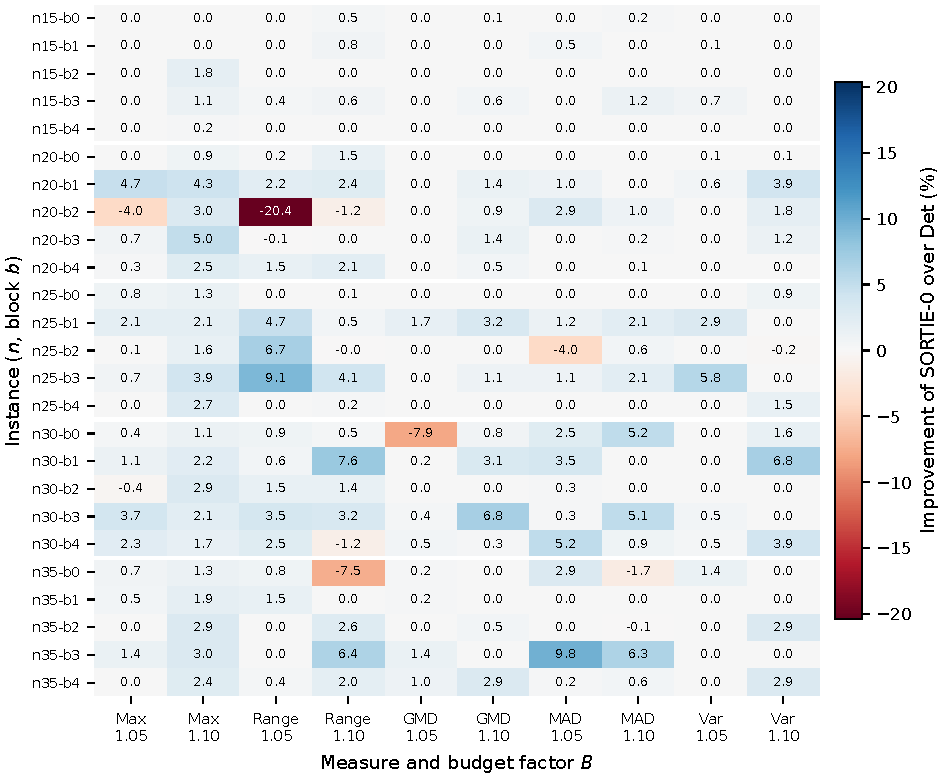
\includegraphics[width=0.9\textwidth]{fig_heatmap_e3.pdf}
\caption{E3: improvement of the ex-post value of SORTIE-0 over Det (\%) for
every instance, measure and budget.}\label{fig:heatmap}
\end{figure}

Tables~\ref{tab:app_e3_110} and~\ref{tab:app_e3_105} list the out-of-sample
ex-post value of every E3 plan, Table~\ref{tab:app_e7b} the seed means and
standard deviations of E7b, and Table~\ref{tab:app_e17} the E17 values per instance and measure
. Every plan is stored in the released plan cache and can be re-evaluated
with the released simulator.

\begin{small}
\begin{longtable}{llrrrrrrr}
\caption{E3, $B=1.10$: out-of-sample ex-post value of every plan (bold: best); Cost: the cost-optimal plan; S-0/S-1: SORTIE-0/1; Gain: improvement of S-0 over Det; last column: total length of the S-0 plan relative to $C^\ast$.}\label{tab:app_e3_110}\\
\toprule
Instance & Measure & Cost & Det & SAA & S-0 & S-1 & Gain (\%) & $\sum L/C^\ast$\\
\midrule
\endfirsthead
\toprule
Instance & Measure & Cost & Det & SAA & S-0 & S-1 & Gain (\%) & $\sum L/C^\ast$\\
\midrule
\endhead
\bottomrule
\endfoot
n15-b0 & Max & 2,640 & 2,547 & 2,561 & 2,547 & \textbf{2,545} & +0.00 & 1.026 \\
 & Range & 2,412 & 1,575 & \textbf{1,568} & \textbf{1,568} & 1,573 & +0.47 & 1.098 \\
 & GMD & 907 & 625 & 625 & 625 & \textbf{623} & +0.06 & 1.100 \\
 & MAD & 652 & 468 & \textbf{467} & \textbf{467} & 467 & +0.20 & 1.100 \\
 & Var & 730,909 & 357,317 & 357,317 & 357,238 & \textbf{354,022} & +0.02 & 1.100 \\
n15-b1 & Max & 2,165 & 2,091 & 2,095 & \textbf{2,091} & \textbf{2,091} & +0.00 & 1.098 \\
 & Range & 1,875 & 1,295 & \textbf{1,285} & \textbf{1,285} & \textbf{1,285} & +0.79 & 1.095 \\
 & GMD & 729 & \textbf{530} & \textbf{530} & \textbf{530} & \textbf{530} & +0.00 & 1.095 \\
 & MAD & 537 & \textbf{405} & \textbf{405} & \textbf{405} & \textbf{405} & +0.00 & 1.095 \\
 & Var & 461,317 & \textbf{258,741} & 261,374 & \textbf{258,741} & \textbf{258,741} & +0.00 & 1.095 \\
n15-b2 & Max & 2,419 & 2,419 & 2,376 & \textbf{2,376} & \textbf{2,376} & +1.78 & 1.070 \\
 & Range & 2,187 & \textbf{1,231} & 1,234 & \textbf{1,231} & \textbf{1,231} & +0.00 & 1.081 \\
 & GMD & 804 & \textbf{478} & 482 & \textbf{478} & 479 & +0.00 & 1.099 \\
 & MAD & 568 & \textbf{347} & \textbf{347} & \textbf{347} & 348 & +0.00 & 1.099 \\
 & Var & 604,666 & \textbf{222,814} & 223,451 & \textbf{222,814} & 223,451 & +0.00 & 1.099 \\
n15-b3 & Max & 1,926 & 1,826 & 1,826 & 1,805 & \textbf{1,803} & +1.13 & 1.070 \\
 & Range & 1,899 & 784 & 806 & 779 & \textbf{773} & +0.64 & 1.070 \\
 & GMD & 665 & 305 & 305 & 303 & \textbf{300} & +0.59 & 1.070 \\
 & MAD & 452 & 226 & 224 & 223 & \textbf{221} & +1.15 & 1.070 \\
 & Var & 471,206 & 90,921 & 95,342 & 90,921 & \textbf{89,222} & +0.00 & 1.095 \\
n15-b4 & Max & 2,412 & 1,940 & \textbf{1,934} & 1,935 & 1,935 & +0.25 & 1.056 \\
 & Range & 2,170 & \textbf{1,024} & \textbf{1,024} & \textbf{1,024} & \textbf{1,024} & +0.00 & 1.098 \\
 & GMD & 772 & \textbf{417} & \textbf{417} & \textbf{417} & \textbf{417} & +0.00 & 1.098 \\
 & MAD & 531 & \textbf{316} & \textbf{316} & \textbf{316} & \textbf{316} & +0.00 & 1.098 \\
 & Var & 543,628 & \textbf{164,264} & \textbf{164,264} & \textbf{164,264} & \textbf{164,264} & +0.00 & 1.098 \\
n20-b0 & Max & 2,656 & 2,651 & 2,647 & \textbf{2,628} & \textbf{2,628} & +0.90 & 1.081 \\
 & Range & 2,428 & 1,549 & 1,537 & 1,526 & \textbf{1,522} & +1.48 & 1.097 \\
 & GMD & 926 & 628 & 631 & 628 & \textbf{626} & +0.00 & 1.099 \\
 & MAD & 672 & 477 & 481 & 477 & \textbf{477} & +0.00 & 1.099 \\
 & Var & 782,670 & 358,873 & 361,706 & 358,394 & \textbf{356,722} & +0.13 & 1.097 \\
n20-b1 & Max & 1,756 & 1,743 & \textbf{1,668} & 1,669 & 1,669 & +4.28 & 1.037 \\
 & Range & 1,332 & 563 & 562 & 550 & \textbf{550} & +2.42 & 1.099 \\
 & GMD & 472 & 217 & 217 & 214 & \textbf{214} & +1.40 & 1.077 \\
 & MAD & 323 & 157 & 159 & \textbf{157} & \textbf{157} & +0.04 & 1.077 \\
 & Var & 230,329 & 47,975 & 47,125 & \textbf{46,117} & \textbf{46,117} & +3.87 & 1.077 \\
n20-b2 & Max & 2,393 & 2,224 & 2,177 & \textbf{2,158} & \textbf{2,158} & +2.97 & 1.096 \\
 & Range & 2,309 & \textbf{1,283} & \textbf{1,283} & 1,299 & 1,293 & -1.24 & 1.090 \\
 & GMD & 886 & 558 & \textbf{552} & 553 & 553 & +0.92 & 1.099 \\
 & MAD & 645 & 387 & \textbf{383} & 383 & 383 & +1.02 & 1.099 \\
 & Var & 692,985 & 257,489 & \textbf{252,913} & \textbf{252,913} & \textbf{252,913} & +1.78 & 1.098 \\
n20-b3 & Max & 2,668 & 2,472 & 2,349 & \textbf{2,348} & \textbf{2,348} & +5.02 & 1.084 \\
 & Range & 2,518 & \textbf{1,272} & 1,278 & \textbf{1,272} & \textbf{1,272} & +0.00 & 1.100 \\
 & GMD & 918 & 523 & 517 & \textbf{516} & 523 & +1.42 & 1.099 \\
 & MAD & 644 & 373 & \textbf{372} & \textbf{372} & 374 & +0.17 & 1.099 \\
 & Var & 757,430 & 250,084 & 247,116 & 247,116 & \textbf{245,946} & +1.19 & 1.098 \\
n20-b4 & Max & 1,981 & 1,823 & 1,782 & 1,778 & \textbf{1,776} & +2.48 & 1.068 \\
 & Range & 1,472 & 1,085 & 1,066 & 1,062 & \textbf{1,060} & +2.13 & 1.068 \\
 & GMD & 617 & 399 & 398 & 397 & \textbf{396} & +0.52 & 1.067 \\
 & MAD & 477 & 282 & \textbf{282} & \textbf{282} & \textbf{282} & +0.14 & 1.098 \\
 & Var & 332,502 & 147,358 & 148,357 & 147,358 & \textbf{146,846} & +0.00 & 1.067 \\
n25-b0 & Max & 2,607 & 2,622 & 2,613 & \textbf{2,588} & \textbf{2,588} & +1.30 & 1.095 \\
 & Range & 2,379 & 1,253 & 1,260 & \textbf{1,252} & 1,253 & +0.11 & 1.100 \\
 & GMD & 858 & \textbf{506} & 508 & \textbf{506} & 507 & +0.00 & 1.100 \\
 & MAD & 597 & 381 & 383 & 381 & \textbf{381} & +0.00 & 1.100 \\
 & Var & 718,676 & 245,392 & 248,480 & \textbf{243,295} & \textbf{243,295} & +0.85 & 1.099 \\
n25-b1 & Max & 2,145 & 1,971 & 1,939 & \textbf{1,931} & \textbf{1,931} & +2.05 & 1.027 \\
 & Range & 1,257 & 618 & 615 & 615 & \textbf{611} & +0.54 & 1.098 \\
 & GMD & 535 & 247 & 238 & 239 & \textbf{236} & +3.19 & 1.098 \\
 & MAD & 417 & 179 & 176 & 175 & \textbf{173} & +2.08 & 1.098 \\
 & Var & 255,701 & 58,275 & 60,272 & 58,275 & \textbf{57,003} & +0.00 & 1.098 \\
n25-b2 & Max & 2,148 & 2,065 & 2,035 & \textbf{2,033} & \textbf{2,033} & +1.56 & 1.097 \\
 & Range & 2,036 & \textbf{1,312} & 1,312 & 1,312 & 1,312 & -0.01 & 1.099 \\
 & GMD & 763 & 539 & 539 & 539 & \textbf{537} & +0.00 & 1.092 \\
 & MAD & 546 & 412 & 409 & 409 & \textbf{408} & +0.62 & 1.092 \\
 & Var & 516,255 & 265,863 & 267,817 & 266,385 & \textbf{264,172} & -0.20 & 1.099 \\
n25-b3 & Max & 1,984 & 2,025 & 1,958 & \textbf{1,946} & \textbf{1,946} & +3.90 & 1.097 \\
 & Range & 1,474 & 874 & 840 & 838 & \textbf{836} & +4.13 & 1.099 \\
 & GMD & 560 & 331 & 333 & \textbf{328} & 331 & +1.06 & 1.098 \\
 & MAD & 405 & 248 & 244 & \textbf{242} & \textbf{242} & +2.15 & 1.098 \\
 & Var & 283,090 & \textbf{104,507} & 107,279 & \textbf{104,507} & 105,353 & +0.00 & 1.098 \\
n25-b4 & Max & 2,151 & 2,197 & 2,143 & 2,137 & \textbf{2,137} & +2.74 & 1.099 \\
 & Range & 1,931 & 1,002 & 1,004 & 999 & \textbf{994} & +0.21 & 1.099 \\
 & GMD & 683 & 393 & 394 & 393 & \textbf{391} & +0.00 & 1.100 \\
 & MAD & 468 & 291 & 292 & 291 & \textbf{290} & +0.00 & 1.100 \\
 & Var & 459,013 & 152,985 & 153,860 & 150,758 & \textbf{149,397} & +1.46 & 1.099 \\
n30-b0 & Max & 2,773 & 2,615 & 2,587 & \textbf{2,585} & \textbf{2,585} & +1.14 & 1.050 \\
 & Range & 2,626 & 1,229 & 1,228 & 1,223 & \textbf{1,223} & +0.47 & 1.099 \\
 & GMD & 1,000 & 497 & 497 & \textbf{493} & 493 & +0.79 & 1.099 \\
 & MAD & 724 & 392 & 372 & \textbf{371} & 372 & +5.22 & 1.099 \\
 & Var & 911,746 & 235,555 & 233,126 & \textbf{231,861} & \textbf{231,861} & +1.57 & 1.099 \\
n30-b1 & Max & 2,657 & 2,574 & 2,540 & \textbf{2,516} & 2,521 & +2.23 & 1.075 \\
 & Range & 2,287 & 1,537 & 1,421 & \textbf{1,420} & \textbf{1,420} & +7.63 & 1.095 \\
 & GMD & 913 & 568 & 551 & 551 & \textbf{550} & +3.06 & 1.100 \\
 & MAD & 684 & 411 & \textbf{409} & 411 & 412 & +0.00 & 1.098 \\
 & Var & 730,545 & 297,591 & 298,366 & 277,261 & \textbf{275,214} & +6.83 & 1.095 \\
n30-b2 & Max & 1,957 & 1,838 & 1,784 & 1,784 & \textbf{1,783} & +2.94 & 1.078 \\
 & Range & 1,838 & 1,002 & 988 & 988 & \textbf{961} & +1.44 & 1.091 \\
 & GMD & 667 & 365 & 372 & 365 & \textbf{365} & +0.00 & 1.091 \\
 & MAD & 466 & 259 & 263 & 259 & \textbf{259} & +0.00 & 1.091 \\
 & Var & 419,940 & 126,369 & 126,369 & 126,369 & \textbf{126,081} & +0.00 & 1.091 \\
n30-b3 & Max & 2,401 & 2,350 & 2,307 & \textbf{2,300} & \textbf{2,300} & +2.13 & 1.097 \\
 & Range & 2,371 & 1,264 & \textbf{1,223} & \textbf{1,223} & 1,284 & +3.25 & 1.100 \\
 & GMD & 853 & 532 & 502 & \textbf{496} & 500 & +6.75 & 1.100 \\
 & MAD & 592 & 396 & \textbf{369} & 375 & \textbf{369} & +5.12 & 1.100 \\
 & Var & 717,888 & \textbf{225,491} & 229,750 & \textbf{225,491} & 228,530 & +0.00 & 1.100 \\
n30-b4 & Max & 2,325 & 2,231 & 2,196 & 2,193 & \textbf{2,191} & +1.69 & 1.068 \\
 & Range & 2,100 & \textbf{1,217} & 1,237 & 1,232 & 1,231 & -1.21 & 1.093 \\
 & GMD & 762 & 494 & 502 & 493 & \textbf{492} & +0.27 & 1.098 \\
 & MAD & 533 & 347 & 351 & 344 & \textbf{344} & +0.90 & 1.100 \\
 & Var & 536,206 & 225,051 & 219,695 & \textbf{216,280} & 225,293 & +3.90 & 1.099 \\
n35-b0 & Max & 2,892 & 2,717 & 2,704 & \textbf{2,682} & \textbf{2,682} & +1.27 & 1.098 \\
 & Range & 2,744 & \textbf{1,376} & 1,741 & 1,479 & 1,724 & -7.46 & 1.096 \\
 & GMD & 1,013 & \textbf{529} & 609 & \textbf{529} & 609 & +0.00 & 1.100 \\
 & MAD & 718 & 421 & 429 & 428 & \textbf{385} & -1.72 & 1.098 \\
 & Var & 964,248 & \textbf{259,530} & 372,532 & \textbf{259,530} & 368,171 & +0.00 & 1.100 \\
n35-b1 & Max & 2,543 & 2,127 & 2,090 & \textbf{2,087} & \textbf{2,087} & +1.91 & 1.096 \\
 & Range & 2,429 & \textbf{825} & \textbf{825} & \textbf{825} & \textbf{825} & +0.00 & 1.098 \\
 & GMD & 946 & \textbf{323} & 324 & \textbf{323} & \textbf{323} & +0.00 & 1.098 \\
 & MAD & 696 & \textbf{238} & 239 & \textbf{238} & \textbf{238} & +0.00 & 1.098 \\
 & Var & 758,306 & \textbf{102,506} & 102,787 & \textbf{102,506} & \textbf{102,506} & +0.00 & 1.098 \\
n35-b2 & Max & 1,922 & 1,794 & 1,742 & \textbf{1,741} & 1,814 & +2.91 & 1.061 \\
 & Range & 1,526 & 553 & 546 & \textbf{538} & \textbf{538} & +2.61 & 1.093 \\
 & GMD & 562 & 209 & \textbf{208} & \textbf{208} & \textbf{208} & +0.48 & 1.093 \\
 & MAD & 398 & \textbf{153} & 153 & 153 & 153 & -0.06 & 1.093 \\
 & Var & 296,372 & 43,908 & 43,424 & \textbf{42,644} & \textbf{42,644} & +2.88 & 1.095 \\
n35-b3 & Max & 2,527 & 2,452 & 2,398 & 2,379 & \textbf{2,379} & +2.98 & 1.100 \\
 & Range & 2,137 & 1,066 & 1,012 & \textbf{998} & \textbf{998} & +6.37 & 1.100 \\
 & GMD & 780 & \textbf{377} & 381 & \textbf{377} & \textbf{377} & +0.00 & 1.100 \\
 & MAD & 548 & 291 & 273 & 273 & \textbf{273} & +6.35 & 1.100 \\
 & Var & 555,805 & \textbf{142,628} & 144,945 & \textbf{142,628} & \textbf{142,628} & +0.00 & 1.100 \\
n35-b4 & Max & 2,510 & 2,186 & 2,142 & \textbf{2,133} & \textbf{2,133} & +2.43 & 1.085 \\
 & Range & 2,436 & 702 & 702 & \textbf{687} & \textbf{687} & +2.03 & 1.097 \\
 & GMD & 902 & 272 & 275 & \textbf{264} & \textbf{264} & +2.92 & 1.097 \\
 & MAD & 640 & 194 & \textbf{193} & \textbf{193} & \textbf{193} & +0.58 & 1.097 \\
 & Var & 772,452 & 71,590 & 72,810 & \textbf{69,523} & \textbf{69,523} & +2.89 & 1.097 \\
\end{longtable}
\end{small}

\begin{small}
\begin{longtable}{llrrrrrrr}
\caption{E3, $B=1.05$: out-of-sample ex-post value of every plan (bold: best); Cost: the cost-optimal plan; S-0/S-1: SORTIE-0/1; Gain: improvement of S-0 over Det; last column: total length of the S-0 plan relative to $C^\ast$.}\label{tab:app_e3_105}\\
\toprule
Instance & Measure & Cost & Det & SAA & S-0 & S-1 & Gain (\%) & $\sum L/C^\ast$\\
\midrule
\endfirsthead
\toprule
Instance & Measure & Cost & Det & SAA & S-0 & S-1 & Gain (\%) & $\sum L/C^\ast$\\
\midrule
\endhead
\bottomrule
\endfoot
n15-b0 & Max & 2,640 & \textbf{2,547} & 2,559 & \textbf{2,547} & \textbf{2,547} & +0.00 & 1.026 \\
 & Range & 2,412 & \textbf{2,319} & 2,331 & \textbf{2,319} & \textbf{2,319} & +0.00 & 1.026 \\
 & GMD & 907 & \textbf{868} & 873 & \textbf{868} & \textbf{868} & +0.00 & 1.026 \\
 & MAD & 652 & \textbf{621} & \textbf{621} & \textbf{621} & \textbf{621} & +0.00 & 1.026 \\
 & Var & 730,909 & \textbf{691,734} & 699,905 & \textbf{691,734} & \textbf{691,734} & +0.00 & 1.026 \\
n15-b1 & Max & 2,165 & \textbf{2,091} & \textbf{2,091} & \textbf{2,091} & \textbf{2,091} & +0.00 & 1.041 \\
 & Range & 1,875 & \textbf{1,503} & \textbf{1,503} & \textbf{1,503} & 1,505 & +0.00 & 1.040 \\
 & GMD & 729 & \textbf{616} & \textbf{616} & \textbf{616} & 617 & +0.00 & 1.040 \\
 & MAD & 537 & 469 & 469 & \textbf{467} & 468 & +0.50 & 1.048 \\
 & Var & 461,317 & 337,238 & 339,053 & \textbf{336,907} & 337,815 & +0.10 & 1.048 \\
n15-b2 & Max & 2,419 & \textbf{2,419} & \textbf{2,419} & \textbf{2,419} & \textbf{2,419} & +0.00 & 1.000 \\
 & Range & 2,187 & \textbf{2,187} & \textbf{2,187} & \textbf{2,187} & \textbf{2,187} & +0.00 & 1.000 \\
 & GMD & 804 & \textbf{804} & \textbf{804} & \textbf{804} & \textbf{804} & +0.00 & 1.000 \\
 & MAD & 568 & \textbf{568} & \textbf{568} & \textbf{568} & \textbf{568} & +0.00 & 1.000 \\
 & Var & 604,666 & \textbf{604,666} & \textbf{604,666} & \textbf{604,666} & \textbf{604,666} & +0.00 & 1.000 \\
n15-b3 & Max & 1,926 & \textbf{1,926} & \textbf{1,926} & \textbf{1,926} & \textbf{1,926} & +0.00 & 1.000 \\
 & Range & 1,899 & 1,181 & \textbf{1,177} & \textbf{1,177} & \textbf{1,177} & +0.37 & 1.043 \\
 & GMD & 665 & 468 & \textbf{468} & 468 & 468 & +0.00 & 1.041 \\
 & MAD & 452 & \textbf{349} & 349 & \textbf{349} & \textbf{349} & +0.00 & 1.041 \\
 & Var & 471,206 & 200,220 & \textbf{198,775} & \textbf{198,775} & \textbf{198,775} & +0.72 & 1.043 \\
n15-b4 & Max & 2,412 & \textbf{1,940} & \textbf{1,940} & \textbf{1,940} & \textbf{1,940} & +0.00 & 1.000 \\
 & Range & 2,170 & \textbf{1,698} & \textbf{1,698} & \textbf{1,698} & \textbf{1,698} & +0.00 & 1.000 \\
 & GMD & 772 & \textbf{648} & \textbf{648} & \textbf{648} & \textbf{648} & +0.00 & 1.022 \\
 & MAD & 531 & \textbf{466} & \textbf{466} & \textbf{466} & \textbf{466} & +0.00 & 1.022 \\
 & Var & 543,628 & \textbf{375,246} & \textbf{375,246} & \textbf{375,246} & \textbf{375,246} & +0.00 & 1.000 \\
n20-b0 & Max & 2,656 & \textbf{2,639} & 2,647 & \textbf{2,639} & \textbf{2,639} & +0.00 & 1.021 \\
 & Range & 2,428 & 2,411 & 2,418 & \textbf{2,405} & \textbf{2,405} & +0.25 & 1.022 \\
 & GMD & 926 & \textbf{863} & \textbf{863} & \textbf{863} & \textbf{863} & +0.00 & 1.049 \\
 & MAD & 672 & \textbf{595} & \textbf{595} & \textbf{595} & \textbf{595} & +0.00 & 1.049 \\
 & Var & 782,670 & 748,918 & 751,999 & \textbf{748,239} & \textbf{748,239} & +0.09 & 1.022 \\
n20-b1 & Max & 1,756 & 1,751 & \textbf{1,668} & 1,669 & 1,669 & +4.72 & 1.037 \\
 & Range & 1,332 & 666 & \textbf{652} & \textbf{652} & \textbf{652} & +2.20 & 1.036 \\
 & GMD & 472 & 251 & \textbf{251} & 251 & 251 & +0.00 & 1.049 \\
 & MAD & 323 & 185 & 184 & \textbf{183} & \textbf{183} & +0.99 & 1.049 \\
 & Var & 230,329 & 62,141 & \textbf{61,759} & \textbf{61,759} & \textbf{61,759} & +0.62 & 1.036 \\
n20-b2 & Max & 2,393 & \textbf{2,191} & 2,202 & 2,279 & 2,279 & -4.03 & 1.039 \\
 & Range & 2,309 & \textbf{1,652} & 1,988 & 1,988 & 1,988 & -20.38 & 1.039 \\
 & GMD & 886 & \textbf{656} & \textbf{656} & \textbf{656} & \textbf{656} & +0.00 & 1.049 \\
 & MAD & 645 & 505 & \textbf{490} & \textbf{490} & \textbf{490} & +2.92 & 1.049 \\
 & Var & 692,985 & \textbf{379,751} & \textbf{379,751} & \textbf{379,751} & \textbf{379,751} & +0.00 & 1.049 \\
n20-b3 & Max & 2,668 & 2,398 & \textbf{2,381} & \textbf{2,381} & \textbf{2,381} & +0.71 & 1.046 \\
 & Range & 2,518 & \textbf{1,640} & 1,642 & 1,642 & 1,642 & -0.10 & 1.044 \\
 & GMD & 918 & \textbf{673} & \textbf{673} & \textbf{673} & \textbf{673} & +0.00 & 1.046 \\
 & MAD & 644 & \textbf{490} & \textbf{490} & \textbf{490} & \textbf{490} & +0.00 & 1.046 \\
 & Var & 757,430 & \textbf{408,393} & \textbf{408,393} & \textbf{408,393} & \textbf{408,393} & +0.00 & 1.046 \\
n20-b4 & Max & 1,981 & 1,819 & \textbf{1,814} & \textbf{1,814} & 1,815 & +0.30 & 1.050 \\
 & Range & 1,472 & 1,235 & \textbf{1,216} & \textbf{1,216} & \textbf{1,216} & +1.51 & 1.047 \\
 & GMD & 617 & \textbf{485} & \textbf{485} & \textbf{485} & \textbf{485} & +0.00 & 1.048 \\
 & MAD & 477 & \textbf{341} & \textbf{341} & \textbf{341} & \textbf{341} & +0.00 & 1.048 \\
 & Var & 332,502 & 208,876 & 208,876 & 208,876 & \textbf{208,721} & +0.00 & 1.045 \\
n25-b0 & Max & 2,607 & 2,610 & 2,613 & \textbf{2,589} & \textbf{2,589} & +0.81 & 1.019 \\
 & Range & 2,379 & \textbf{1,755} & \textbf{1,755} & \textbf{1,755} & \textbf{1,755} & +0.00 & 1.050 \\
 & GMD & 858 & \textbf{683} & \textbf{683} & \textbf{683} & \textbf{683} & +0.00 & 1.050 \\
 & MAD & 597 & \textbf{503} & \textbf{503} & \textbf{503} & \textbf{503} & +0.00 & 1.050 \\
 & Var & 718,676 & \textbf{416,021} & \textbf{416,021} & \textbf{416,021} & \textbf{416,021} & +0.00 & 1.050 \\
n25-b1 & Max & 2,145 & 1,971 & 1,938 & \textbf{1,931} & \textbf{1,931} & +2.05 & 1.027 \\
 & Range & 1,257 & 774 & 745 & \textbf{738} & \textbf{738} & +4.66 & 1.027 \\
 & GMD & 535 & 290 & 288 & \textbf{285} & \textbf{285} & +1.69 & 1.027 \\
 & MAD & 417 & 212 & 211 & \textbf{209} & \textbf{209} & +1.22 & 1.027 \\
 & Var & 255,701 & 82,851 & 81,533 & \textbf{80,430} & \textbf{80,430} & +2.92 & 1.027 \\
n25-b2 & Max & 2,148 & 2,148 & 2,147 & \textbf{2,145} & \textbf{2,145} & +0.13 & 1.029 \\
 & Range & 2,036 & 1,815 & \textbf{1,693} & \textbf{1,693} & \textbf{1,693} & +6.71 & 1.046 \\
 & GMD & 763 & \textbf{654} & \textbf{654} & \textbf{654} & 689 & +0.00 & 1.046 \\
 & MAD & 546 & \textbf{479} & 504 & 498 & \textbf{479} & -3.99 & 1.040 \\
 & Var & 516,255 & 418,916 & \textbf{372,661} & 418,916 & 417,741 & +0.00 & 1.036 \\
n25-b3 & Max & 1,984 & 1,968 & 1,958 & \textbf{1,953} & \textbf{1,953} & +0.72 & 1.045 \\
 & Range & 1,474 & 1,162 & 1,058 & \textbf{1,056} & \textbf{1,056} & +9.13 & 1.045 \\
 & GMD & 560 & \textbf{419} & 423 & \textbf{419} & \textbf{419} & +0.00 & 1.046 \\
 & MAD & 405 & 314 & 312 & \textbf{311} & \textbf{311} & +1.10 & 1.050 \\
 & Var & 283,090 & 169,897 & \textbf{160,109} & \textbf{160,109} & \textbf{160,109} & +5.76 & 1.046 \\
n25-b4 & Max & 2,151 & 2,151 & 2,151 & \textbf{2,150} & \textbf{2,150} & +0.03 & 1.044 \\
 & Range & 1,931 & \textbf{1,433} & 1,544 & \textbf{1,433} & 1,544 & +0.00 & 1.034 \\
 & GMD & 683 & \textbf{565} & \textbf{565} & \textbf{565} & \textbf{565} & +0.00 & 1.044 \\
 & MAD & 468 & \textbf{397} & \textbf{397} & \textbf{397} & \textbf{397} & +0.00 & 1.044 \\
 & Var & 459,013 & \textbf{294,618} & \textbf{294,618} & \textbf{294,618} & \textbf{294,618} & +0.00 & 1.044 \\
n30-b0 & Max & 2,773 & 2,606 & 2,602 & \textbf{2,597} & 2,597 & +0.36 & 1.044 \\
 & Range & 2,626 & 2,388 & 2,393 & 2,368 & \textbf{2,357} & +0.86 & 1.044 \\
 & GMD & 1,000 & \textbf{760} & 831 & 820 & 821 & -7.91 & 1.044 \\
 & MAD & 724 & 566 & 551 & 552 & \textbf{548} & +2.54 & 1.044 \\
 & Var & 911,746 & 516,782 & 516,782 & 516,782 & \textbf{515,564} & +0.00 & 1.048 \\
n30-b1 & Max & 2,657 & 2,552 & 2,530 & \textbf{2,524} & 2,526 & +1.13 & 1.037 \\
 & Range & 2,287 & 1,903 & 1,893 & \textbf{1,892} & 1,893 & +0.61 & 1.041 \\
 & GMD & 913 & 759 & 761 & 758 & \textbf{706} & +0.16 & 1.044 \\
 & MAD & 684 & 535 & 516 & \textbf{516} & 517 & +3.54 & 1.049 \\
 & Var & 730,545 & \textbf{460,952} & \textbf{460,952} & \textbf{460,952} & \textbf{460,952} & +0.00 & 1.044 \\
n30-b2 & Max & 1,957 & \textbf{1,942} & 1,958 & 1,950 & 1,949 & -0.39 & 1.034 \\
 & Range & 1,838 & 1,224 & 1,217 & 1,205 & \textbf{1,204} & +1.53 & 1.049 \\
 & GMD & 667 & 508 & 514 & 508 & \textbf{508} & +0.00 & 1.048 \\
 & MAD & 466 & 393 & 393 & \textbf{392} & 394 & +0.28 & 1.049 \\
 & Var & 419,940 & 225,689 & 230,414 & 225,689 & \textbf{225,408} & +0.00 & 1.048 \\
n30-b3 & Max & 2,401 & 2,387 & 2,306 & \textbf{2,300} & \textbf{2,300} & +3.67 & 1.042 \\
 & Range & 2,371 & 1,946 & \textbf{1,878} & \textbf{1,878} & \textbf{1,878} & +3.51 & 1.050 \\
 & GMD & 853 & 664 & \textbf{661} & \textbf{661} & \textbf{661} & +0.39 & 1.050 \\
 & MAD & 592 & 453 & 453 & \textbf{451} & \textbf{451} & +0.32 & 1.050 \\
 & Var & 717,888 & 449,606 & \textbf{447,388} & \textbf{447,388} & \textbf{447,388} & +0.49 & 1.050 \\
n30-b4 & Max & 2,325 & 2,244 & 2,200 & \textbf{2,193} & \textbf{2,193} & +2.28 & 1.045 \\
 & Range & 2,100 & 1,739 & 1,701 & \textbf{1,695} & \textbf{1,695} & +2.53 & 1.043 \\
 & GMD & 762 & 632 & 632 & \textbf{629} & 630 & +0.51 & 1.050 \\
 & MAD & 533 & 457 & \textbf{433} & \textbf{433} & \textbf{433} & +5.16 & 1.048 \\
 & Var & 536,206 & 354,473 & 364,184 & \textbf{352,875} & \textbf{352,875} & +0.45 & 1.046 \\
n35-b0 & Max & 2,892 & 2,717 & 2,703 & 2,697 & \textbf{2,694} & +0.75 & 1.035 \\
 & Range & 2,744 & 2,488 & 2,486 & 2,468 & \textbf{2,447} & +0.80 & 1.035 \\
 & GMD & 1,013 & 846 & 860 & 844 & \textbf{841} & +0.24 & 1.028 \\
 & MAD & 718 & 580 & 574 & 564 & \textbf{562} & +2.88 & 1.028 \\
 & Var & 964,248 & 809,215 & 800,421 & 798,285 & \textbf{793,815} & +1.35 & 1.022 \\
n35-b1 & Max & 2,543 & 2,245 & \textbf{2,137} & 2,233 & \textbf{2,137} & +0.52 & 1.045 \\
 & Range & 2,429 & 1,793 & 1,768 & 1,767 & \textbf{1,239} & +1.48 & 1.049 \\
 & GMD & 946 & 502 & 502 & 501 & \textbf{499} & +0.22 & 1.050 \\
 & MAD & 696 & \textbf{374} & \textbf{374} & \textbf{374} & \textbf{374} & +0.00 & 1.050 \\
 & Var & 758,306 & 228,342 & 230,146 & 228,342 & \textbf{228,317} & +0.00 & 1.050 \\
n35-b2 & Max & 1,922 & \textbf{1,748} & \textbf{1,748} & \textbf{1,748} & \textbf{1,748} & +0.00 & 1.047 \\
 & Range & 1,526 & \textbf{620} & \textbf{620} & \textbf{620} & \textbf{620} & +0.00 & 1.047 \\
 & GMD & 562 & \textbf{246} & \textbf{246} & \textbf{246} & \textbf{246} & +0.00 & 1.047 \\
 & MAD & 398 & \textbf{184} & \textbf{184} & \textbf{184} & \textbf{184} & +0.00 & 1.047 \\
 & Var & 296,372 & \textbf{58,746} & \textbf{58,746} & \textbf{58,746} & \textbf{58,746} & +0.00 & 1.047 \\
n35-b3 & Max & 2,527 & 2,453 & 2,420 & \textbf{2,420} & 2,423 & +1.36 & 1.037 \\
 & Range & 2,137 & \textbf{1,292} & \textbf{1,292} & \textbf{1,292} & \textbf{1,292} & +0.00 & 1.050 \\
 & GMD & 780 & 532 & \textbf{524} & \textbf{524} & \textbf{524} & +1.42 & 1.050 \\
 & MAD & 548 & 440 & \textbf{397} & \textbf{397} & \textbf{397} & +9.77 & 1.050 \\
 & Var & 555,805 & \textbf{247,798} & \textbf{247,798} & \textbf{247,798} & \textbf{247,798} & +0.00 & 1.050 \\
n35-b4 & Max & 2,510 & \textbf{2,153} & 2,174 & \textbf{2,153} & \textbf{2,153} & +0.00 & 1.025 \\
 & Range & 2,436 & 1,026 & \textbf{1,022} & \textbf{1,022} & \textbf{1,022} & +0.38 & 1.050 \\
 & GMD & 902 & 415 & \textbf{411} & \textbf{411} & \textbf{411} & +0.96 & 1.050 \\
 & MAD & 640 & 290 & \textbf{290} & \textbf{290} & \textbf{290} & +0.24 & 1.048 \\
 & Var & 772,452 & \textbf{156,368} & 158,633 & \textbf{156,368} & 158,899 & +0.00 & 1.050 \\
\end{longtable}
\end{small}

\begin{small}
\begin{longtable}{llrrrr}
\caption{E7b, $n=100$: mean (standard deviation) over three solver seeds of the ex-post value.}\label{tab:app_e7b}\\
\toprule
Instance & Measure & Det & SAA & S-0 & S-0 vs Det (\%)\\
\midrule
\endfirsthead
\toprule
Instance & Measure & Det & SAA & S-0 & S-0 vs Det (\%)\\
\midrule
\endhead
\bottomrule
\endfoot
n100-b0 & GMD & 378 (53.9) & 349 (11.7) & 337 (3.7) & +10.77 \\
n100-b0 & Max & 3,016 (137) & 2,930 (6.2) & 2,924 (6.3) & +3.06 \\
n100-b0 & Range & 870 (1.0) & 861 (12.9) & 840 (0.3) & +3.44 \\
n100-b1 & GMD & 249 (30.4) & 231 (1.6) & 235 (4.6) & +5.71 \\
n100-b1 & Max & 2,727 (9.7) & 2,665 (2.7) & 2,667 (0.3) & +2.20 \\
n100-b1 & Range & 604 (3.5) & 648 (27.8) & 610 (8.6) & -1.05 \\
n100-b2 & GMD & 346 (17.6) & 351 (6.7) & 401 (39.8) & -15.87 \\
n100-b2 & Max & 2,444 (8.5) & 2,493 (32.0) & 2,484 (62.5) & -1.65 \\
n100-b2 & Range & 1,081 (318) & 929 (44.4) & 970 (5.4) & +10.26 \\
n100-b3 & GMD & 304 (10.3) & 313 (14.9) & 305 (7.8) & -0.20 \\
n100-b3 & Max & 2,583 (51.7) & 2,535 (0.2) & 2,602 (117) & -0.72 \\
n100-b3 & Range & 881 (10.6) & 785 (7.3) & 799 (9.8) & +9.35 \\
n100-b4 & GMD & 516 (5.5) & 523 (19.8) & 502 (11.3) & +2.79 \\
n100-b4 & Max & 2,525 (8.6) & 2,497 (12.4) & 2,475 (15.8) & +2.02 \\
n100-b4 & Range & 1,346 (64.1) & 1,365 (63.8) & 1,335 (50.6) & +0.83 \\
n100-b5 & GMD & 289 (6.6) & 273 (4.1) & 243 (22.8) & +15.89 \\
n100-b5 & Max & 2,396 (12.8) & 2,431 (62.3) & 2,391 (8.5) & +0.23 \\
n100-b5 & Range & 890 (282) & 700 (85.3) & 630 (69.9) & +29.24 \\
\end{longtable}
\end{small}

\begin{small}
\begin{longtable}{llrrrrr}
\caption{E17: ex-post value, mean over two solver seeds (bold: best).}\label{tab:app_e17}\\
\toprule
Instance & Measure & Det & SAA & S-0 & Det-$\sigma$ & S-0 vs Det (\%)\\
\midrule
\endfirsthead
\toprule
Instance & Measure & Det & SAA & S-0 & Det-$\sigma$ & S-0 vs Det (\%)\\
\midrule
\endhead
\bottomrule
\endfoot
X-n101-k25-h50 & GMD & 267 & 268 & \textbf{265} & 279 & +0.65 \\
 & Max & 2,049 & 2,027 & \textbf{2,013} & 2,060 & +1.73 \\
 & Range & 755 & 731 & \textbf{709} & 767 & +6.01 \\
X-n106-k14-h50 & GMD & 499 & 508 & \textbf{497} & 513 & +0.36 \\
 & Max & 2,874 & 2,821 & \textbf{2,811} & 2,869 & +2.19 \\
 & Range & 1,317 & 1,285 & \textbf{1,271} & 1,300 & +3.52 \\
X-n110-k13-h50 & GMD & 154 & 152 & \textbf{148} & 156 & +4.21 \\
 & Max & 1,781 & 1,731 & \textbf{1,728} & 1,751 & +2.97 \\
 & Range & 397 & 392 & \textbf{382} & 395 & +3.76 \\
X-n115-k10-h50 & GMD & 167 & 160 & \textbf{159} & 174 & +4.67 \\
 & Max & 1,788 & 1,790 & \textbf{1,781} & 1,800 & +0.40 \\
 & Range & 409 & 415 & \textbf{405} & 414 & +1.07 \\
X-n120-k6-h50 & GMD & 609 & 662 & \textbf{583} & 636 & +4.32 \\
 & Max & 2,843 & 2,830 & \textbf{2,829} & 2,859 & +0.51 \\
 & Range & 1,493 & 1,499 & \textbf{1,480} & 1,518 & +0.83 \\
X-n125-k30-h50 & GMD & 358 & 359 & \textbf{352} & 365 & +1.69 \\
 & Max & 2,689 & 2,670 & \textbf{2,642} & 2,696 & +1.75 \\
 & Range & 929 & 929 & 916 & \textbf{914} & +1.30 \\
X-n129-k18-h50 & GMD & \textbf{557} & 581 & 565 & 560 & -1.31 \\
 & Max & 2,843 & 2,817 & \textbf{2,795} & 2,842 & +1.69 \\
 & Range & 1,437 & 1,399 & \textbf{1,398} & 1,417 & +2.72 \\
X-n134-k13-h50 & GMD & 460 & \textbf{460} & 460 & 463 & +0.05 \\
 & Max & 1,935 & 1,936 & \textbf{1,894} & 1,986 & +2.08 \\
 & Range & \textbf{1,354} & 1,358 & 1,355 & 1,378 & -0.06 \\
X-n139-k10-h50 & GMD & 173 & 160 & \textbf{159} & 164 & +8.01 \\
 & Max & 1,804 & 1,788 & \textbf{1,785} & 1,792 & +1.07 \\
 & Range & 428 & 413 & \textbf{412} & 432 & +3.63 \\
X-n143-k7-h50 & GMD & 536 & \textbf{535} & 544 & 550 & -1.52 \\
 & Max & 3,087 & 2,979 & \textbf{2,960} & 3,038 & +4.10 \\
 & Range & 1,442 & 1,365 & \textbf{1,352} & 1,482 & +6.24 \\
X-n148-k46-h50 & GMD & \textbf{250} & 252 & 253 & 258 & -0.95 \\
 & Max & 2,087 & 2,021 & \textbf{2,017} & 2,080 & +3.33 \\
 & Range & 600 & 597 & \textbf{583} & 586 & +2.88 \\
X-n153-k22-h50 & GMD & \textbf{177} & 186 & 178 & 188 & -0.54 \\
 & Max & 1,523 & 1,506 & \textbf{1,504} & 1,517 & +1.28 \\
 & Range & 472 & 466 & \textbf{457} & 480 & +3.06 \\
\end{longtable}
\end{small}



\bibliographystyle{apacite}
\bibliography{references}
\end{document}
